
%%%%%%%%% PROPOSAL -- 15 pages (including Prior NSF Support)

\section{Introduction}
In the last decade, our knowledge of the neutrino has grown exponentially. Low-energy neutrino ($\lesssim$10~MeV) experiments have been instrumental in proving that neutrinos oscillate and therefore have mass. Although our picture of the physics is much clearer now, many questions remain. One of the most tantalizing is the question of the Majorana nature of the neutrino, or, stated differently, whether the neutrino is its own antiparticle. If the neutrino is Majorana then, in models of leptogenesis, the neutrino is responsible for the matter-antimatter  asymmetry we observe in the universe today. This is why both the Multidivisional Neutrino Study from 2004\cite{numatrix}  and this year's National Academy report on nuclear physics\cite{national2012Nuclear} highlight this as a key question to be addressed in the next generation of neutrino experiments.

The only feasible experimental probes of the Majorana nature of the neutrino are low-energy neutrino experiments searching for the rare nuclear process neutrinoless double-beta decay (\zeronu). The next generation of these experiments has started to take data, with first results from EXO\cite{EXO2012} and KamLAND-Zen\cite{KZ2nu} presented in the last year. These experiments are designed either to confirm or refute the claimed observation in \isoge\cite{KKK2006}. The first experiment designed to have the sensitivity to push beyond these bounds into the uncharted territory of the inverted neutrino mass hierarchy is the CUORE experiment. 

CUORE is a two-staged experiment, which builds on the experience of the successful CUORICINO experiment\cite{CC2008}. It uses TeO$_{2}$ crystals instrumented as bolometers to search for \zeronu~in \isomain. The first stage of the experiment, CUORE-0, started in the fall of 2012 with the commencement of data taking from the first tower of CUORE crystals. This makes it an excellent time for a young PI to join the experiment, gain experience in this unique detector technology, and make a valuable contribution to both the hardware and the analysis.

The PI of this proposal has considerable experience in low-energy neutrino physics from their work on the KamLAND and Double Chooz experiments. In particular, the PI is very familiar with the modeling of backgrounds from natural radioactivity, in addition to having extensive experience simulating backgrounds produced in muon spallation. The final sensitivity of the \zeronu~analysis depends almost entirely on the understanding of the backgrounds; therefore, this knowledge transfers very effectively to the CUORE analysis.

There are two tasks on CUORE that need more resources as CUORE makes the transition from construction to commissioning and data taking. These are the slow monitoring system and the Monte Carlo (MC). Because CUORE represents a leap forward in size for this technology, the tools developed for CUORICINO for both of these systems are insufficient. The PI performed performed these same job on Double Chooz, so brings experience from commissioning, operating, and analyzing data from that detector, and is well positioned to lead these efforts.    

The hardware and analysis tasks outlined in this proposal fit in nicely with the PI's skills and the project's needs. The group, the PI with  postdoc Dr. Kevin Hickerson, graduate student Erin Hansen and undergraduate Elizabeth Friedman are ready to start the proposed tasks. Furthermore, these tasks complement the work being done at UCLA  by Professor Huan Huang's group on the front-end electronics, and this award would create a quorum for analysis at UCLA. The timescale of the proposed work fits well with the overall schedule of the experiment. In the first year of the grant, the slow monitoring interfaces would be written and the data from CUORE-0 analyzed. In year two of the grant, the full CUORE detector is commissioned, and this is followed by the first results from CUORE in year three of the grant. This schedule, the details of the physics, and the proposed work are outlined further in the body of this proposal.


\section{Motivation}
\subsection{Neutrino Oscillation: Neutrino Mass to Precision Measurements}
The standard model neutrino is a massless particle which comes in three weak flavor eigenstates: electron, muon, and tau. It was realized early on that if the mass eigenstates of the neutrino do not correspond to the interaction states then a classic quantum oscillation scenario develops. Pontecorvo first proposed a neutrino oscillation scenario of  $\nu-\bar{\nu}$, which was similar to the oscillation seen in the quarks with systems like $K^{0}-\bar{K^{0}}$ \cite{Pontecorvo:1957qd}. The flavor oscillations that we now observe correspond to the scenario first outlined by Maki, Nakagawa, and Sakata (MNS)\cite{Maki:1962mu}. 

In the MNS scenario, the flavor eigenstates of the weak interaction are described by the superposition of the mass eigenstates as
\begin{equation}
\left| \nu_{\alpha} \right> = \sum_{j} U^*_{\alpha j} \left| \nu_{j}\right>,
\end{equation}
where the matrix describes the mixing of the mass eigenstates. This matrix U is called the MNSP matrix in honor of the original formulators. It is parameterized by three mixing angles and at least one complex phase, $\delta$:
\begin{equation}
\label{eq:osc_matrix}
\begin{array}{l c l}
U_{\alpha j} & = &
\begin{pmatrix}
1 & 0 & 0 \\
0 & \cos \theta_{23} & \sin \theta_{23}\\ 
0 & -\sin \theta_{23} & \cos \theta_{23} 
\end{pmatrix}
\begin{pmatrix}
\cos \theta_{13} & 0 &  \sin \theta_{13}e^{-i\delta}\\
0 & 1 & 0\\ 
-\sin \theta_{13}e^{i\delta} & 0 & \cos \theta_{13}
\end{pmatrix}
\begin{pmatrix} 
\cos \theta_{12} & \sin \theta_{12}  & 0\\ 
-\sin \theta_{12} & \cos \theta_{12}  & 0\\
0 & 0 & 1
\end{pmatrix} 
\\
\\
 & \times & \begin{pmatrix}
 e^{i\xi_{1}/2} & 0 & 0\\ 
0 & e^{i\xi_{2}/2} & 0\\ 
0 & 0 & 1
\end{pmatrix}
\end{array}.
\end{equation}
The additional complex phases,  $\xi_1$ and $\xi_2$, are only relevant for Majorana neutrinos. 

The discovery of neutrino oscillation and now the precision measurement of the mixing angles with the corresponding mass differences are the two great accomplishments of neutrino oscillation experiments. With the measurement of $\theta_{13}$, all angles in the MNSP matrix are now known. Therefore, the phases are now the main focus of the neutrino community. The only phase that can be measured in an oscillation experiment is $\delta$. The PI has contributed to one proposed experiment, DAE$\delta$ALUS\cite{Alonso:2010fs}, which aims to create a pion decay-at-rest beam using cyclotron technology. The PI has also been involved in the precursor experiment to DAE$\delta$ALUS, IsoDAR, which proposes to uses a smaller cyclotron to make a $^{8}$Li isotope decay-at-rest antineutrino beam to search for sterile neutrinos. This is one future experiment that the group is working on mainly through small undergraduate projects. The PI would like to continue working on these future endeavors; however, the focus of this proposal is the Majorana phases whose combined effect can be observed in \zeronu~experiments. These experiments analyze signals and backgrounds in the 0.5-5~MeV region and it is in this energy range where the PI has the greatest expertise.

\subsection{Neutrinoless Double Beta Decay}

\begin{figure}
\begin{center}
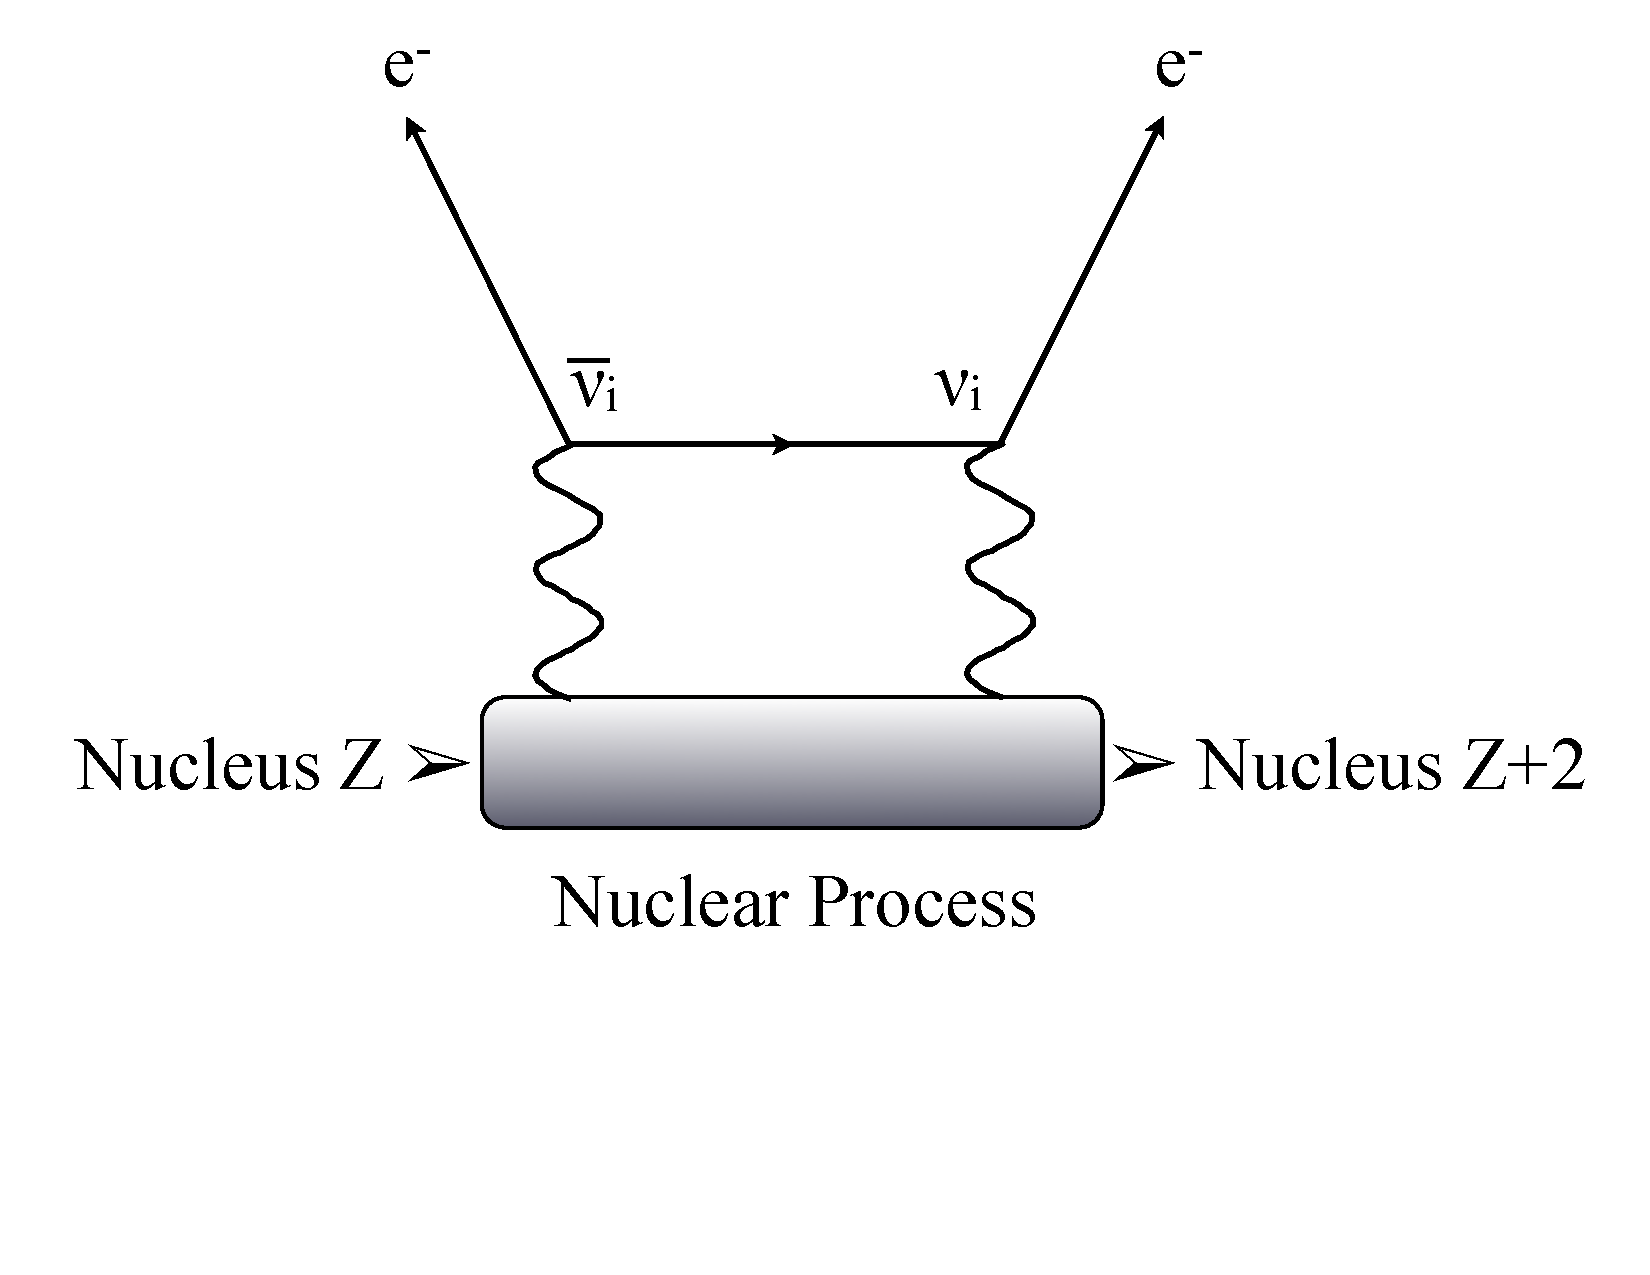
\includegraphics[trim = 0mm 10mm 0mm 5mm, clip, width=0.3\columnwidth]{figs/0nBB.pdf} 
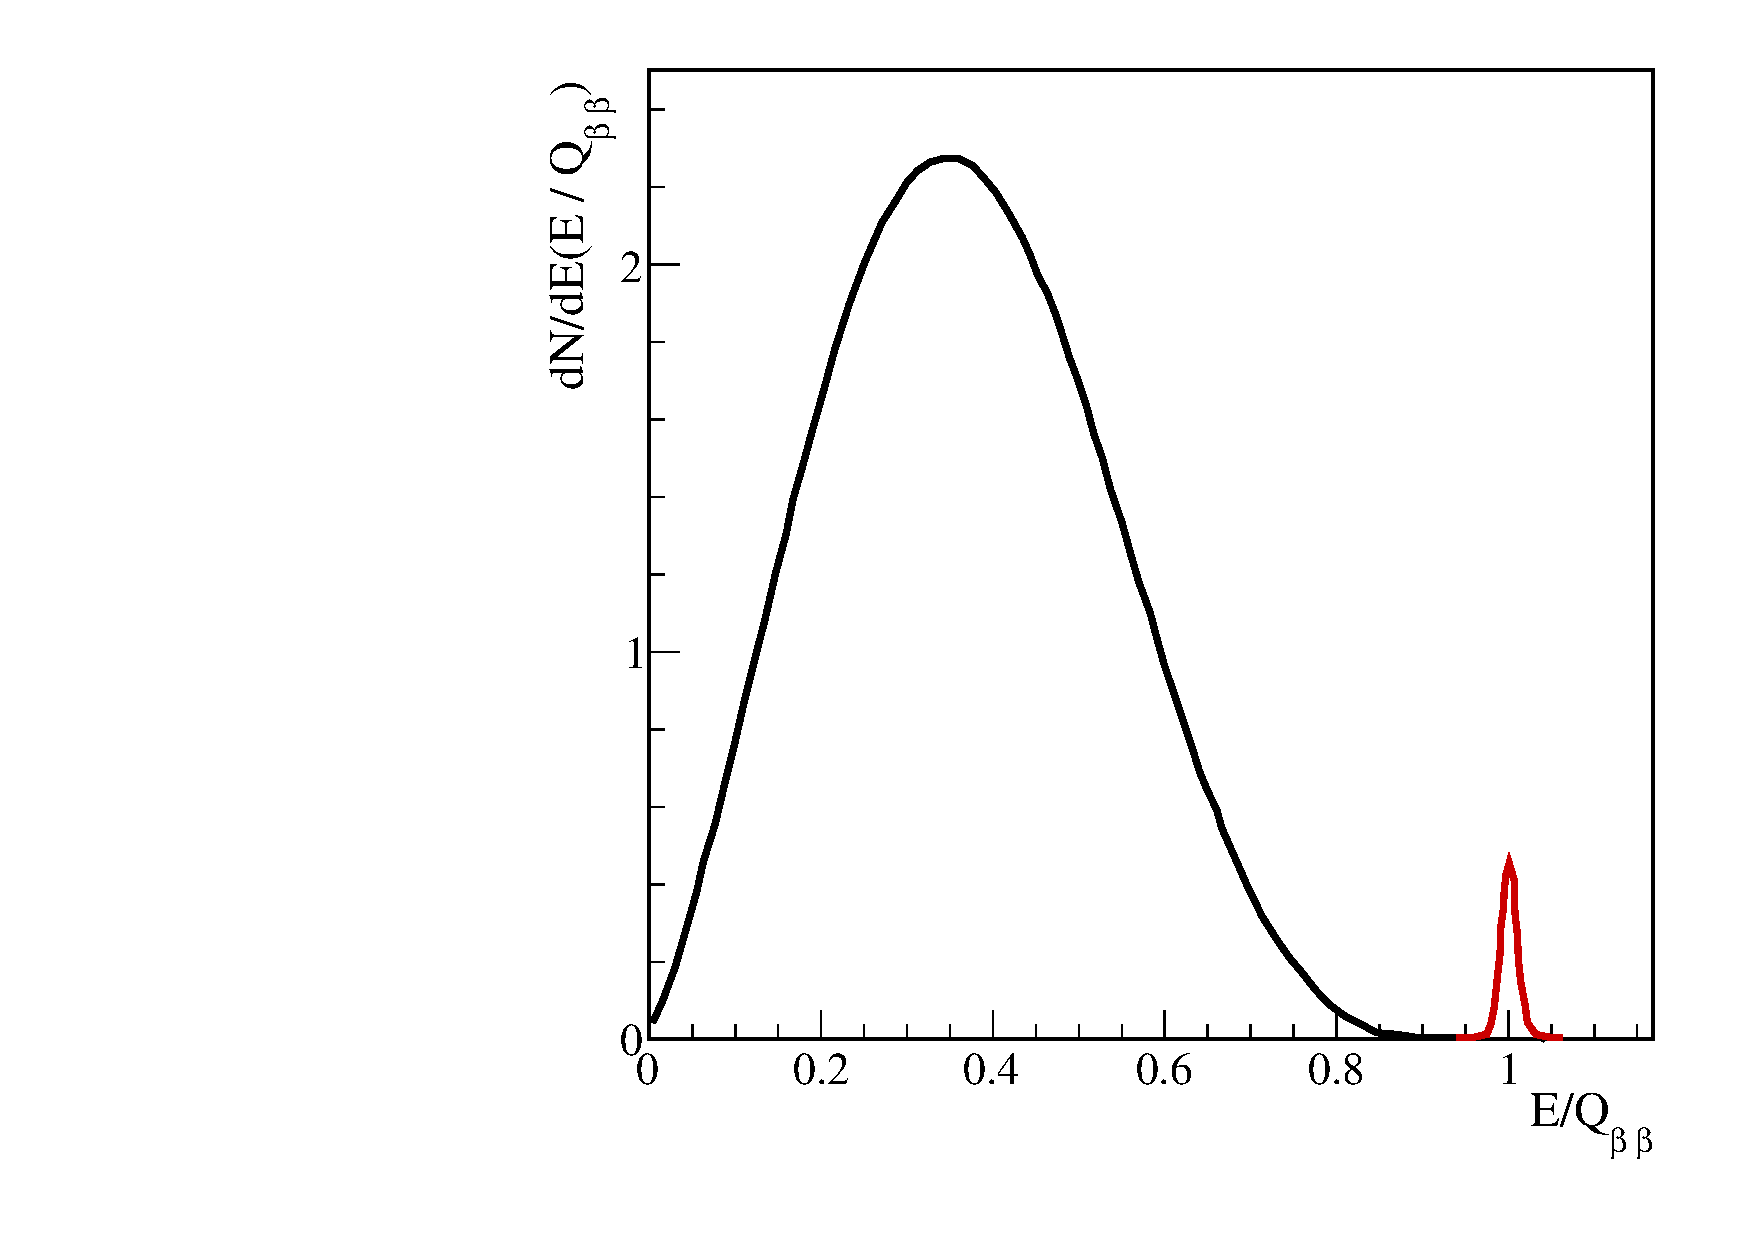
\includegraphics[width=0.25\columnwidth]{figs/CartoonBB.pdf}
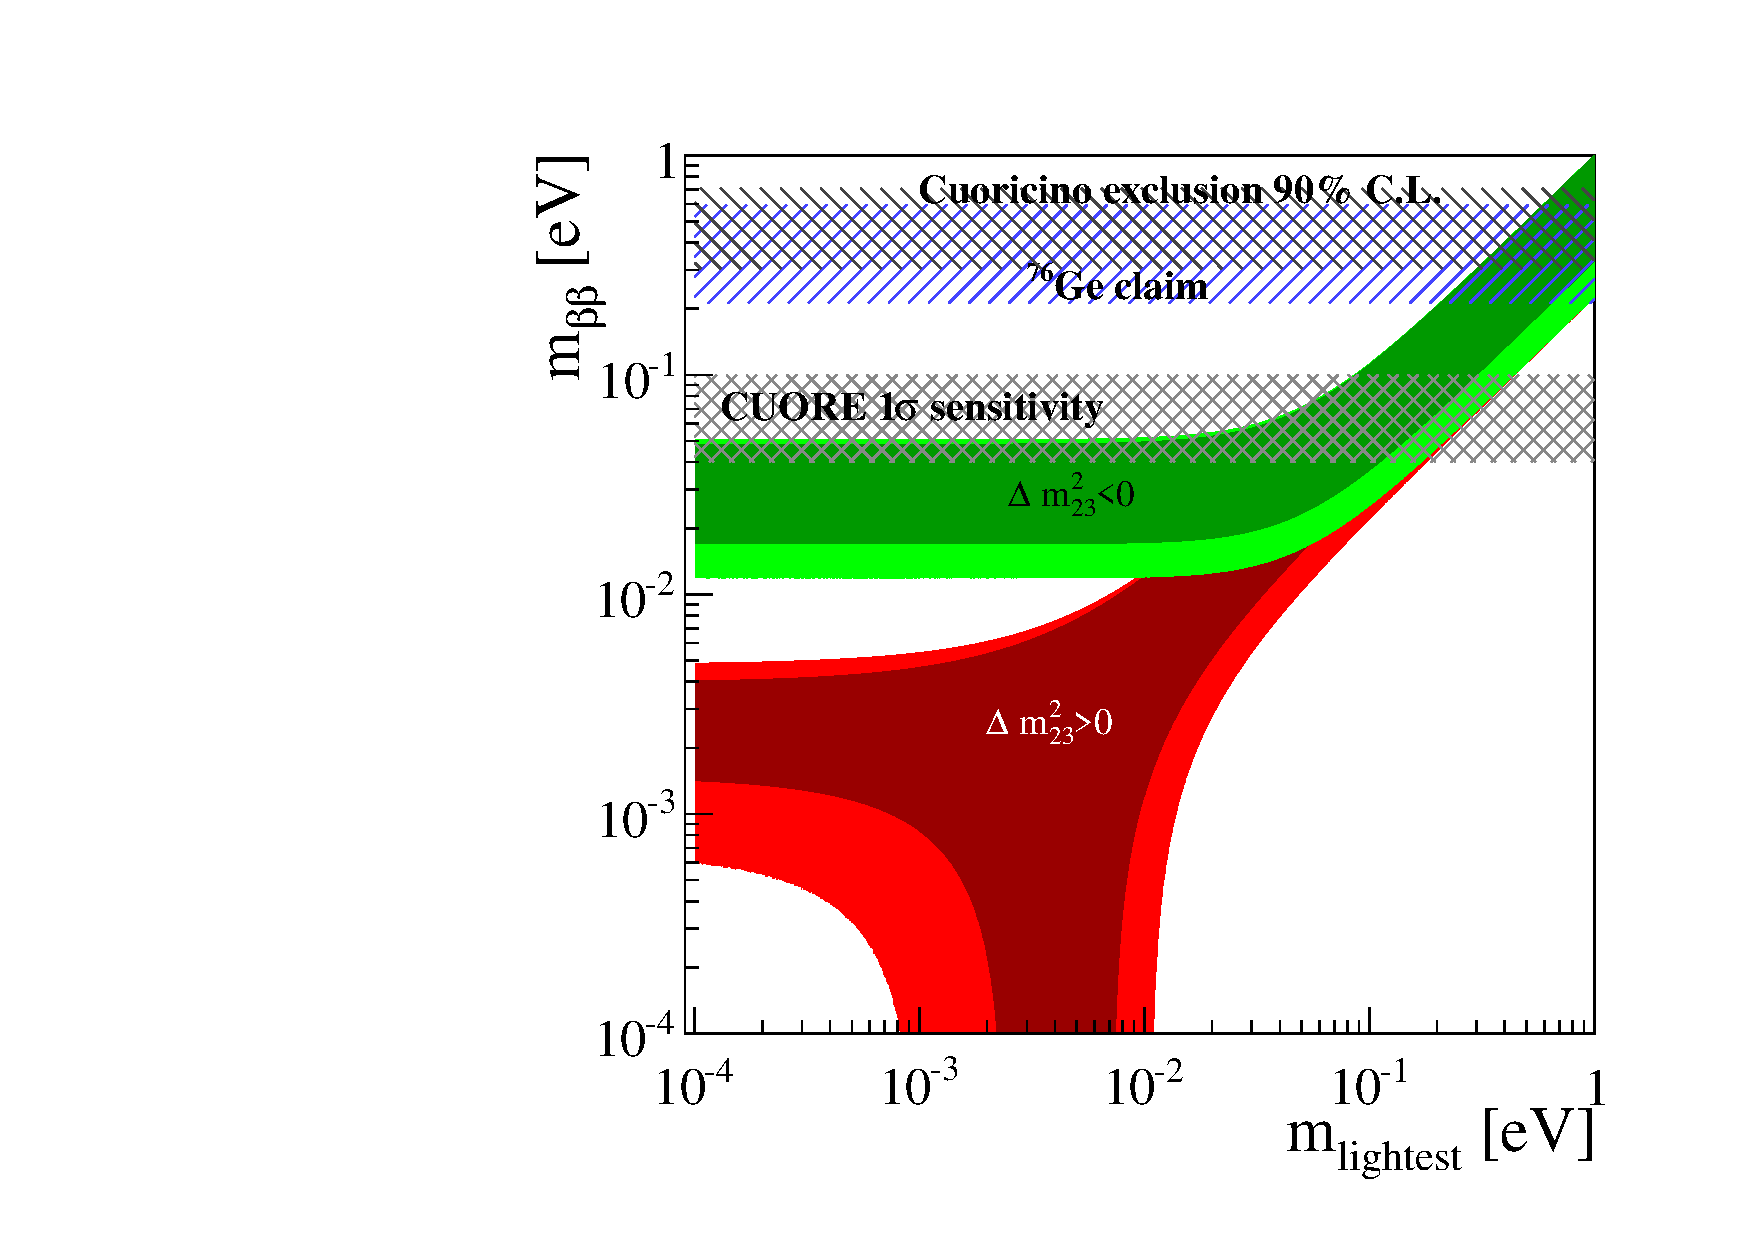
\includegraphics[trim=0.3cm 0.08cm 0.5cm 0.1cm, clip=true, width=0.26\columnwidth]{figs/M_bb_vs_m1_CL-2012.pdf} 
\end{center}
\caption{\footnotesize\label{fig0nuBB}  (Left) Feynman diagram for neutrinoless double-beta decay through light Majorana neutrino exchange. (Middle) Cartoon of the spectrum of electron energies from double-beta decay. The red section at the endpoint $Q_{\beta \beta}$ indicates those from neutrinoless double-beta decay\cite{RevBB}. (Right) The parameter space for \zeronu~as a function of the lightest neutrino mass  and the effective Majorana mass of the neutrinos, $m_{ee}$ \cite{Alessandria:2011rc}. }%The CUORE experiment will be the first to push into the inverted hierarchy. \cite{Alessandria:2011rc}.}
\end{figure}

The main mechanism for \zeronu~is the exchange of a light Majorana neutrino, as shown in Fig.~\ref{fig0nuBB} (Left).  This process is observable in isotopes where the single-beta decay to the Z+1 nucleus is kinematically forbidden so only the double-beta decay to the Z+2 nucleus is possible. The observed signal will be an excess of events at the endpoint of the \twonu~decay spectrum, see Fig.~\ref{fig0nuBB} (Middle). These experiments measure the half-life of  the \zeronu~decay:
\begin{equation}
\label{half0nu}
(T_{1/2}^{0\nu})^{-1} = G_{0\nu}(Q_{\beta\beta}, Z) | M_{0\nu}|^{2} \langle m_{\beta\beta} \rangle^{2}.
\end{equation}
$G_{0\nu}(Q_{\beta\beta}, Z)$ is the phase space available to the decay. $M_{0\nu}$ is the nuclear matrix element  for the decay. The last term is the effective Majorana mass of the neutrino,
\begin{equation}
m_{\beta\beta}= \sum_{i} U^{2}_{e i} m_{i}=\cos^{2}\theta_{13} ( m_{1}e^{2i\xi_2}\cos^{2}\theta_{12} + m_{2}e^{2i\xi_{1}}\sin^{2}\theta_{12})+m_{3}\sin^{2}\theta_{13}
\end{equation}
The sensitivity of \zeronu~experiments is plotted in terms of $m_{\beta\beta}$ versus the lightest neutrino mass eigenstate. Fig.~\ref{fig0nuBB} (right) is the expected sensitivity of the CUORE experiment. The sensitivity has a width due to the uncertainty in the nuclear matrix elements. The parameter space has an intrinsic width due to the interference of the two phases that contribute to \zeronu. There are two distinct regions corresponding to the inverted hierarchy for neutrino mass, the green region in  Fig.~\ref{fig0nuBB} (right)  and that corresponding to the normal hierarchy, the red region in  Fig.~\ref{fig0nuBB} (right). CUORE will be one of the first experiments to push into \zeronu~parameter space for the inverted hierarchy.

The sensitivity shown in Fig.~\ref{fig0nuBB} is the result of a detailed calculation\cite{Alessandria:2011rc}; however,  the sensitivity of a \zeronu~experiment can be approximated as\cite{sens0nu}
\begin{equation}
\label{sens0nu}
T_{1/2}^{0\nu}(n_\sigma) = \frac{4.16\times 10^{26} yr}{n_\sigma} \left ( \frac{\epsilon a}{W} \right ) \sqrt{ \frac{Mt}{b\Delta(E)}}.
\end{equation}
In this approximation, $n_\sigma$ is the number of standard deviations for the resulting half-life, $\epsilon$ is the detector efficiency, a is the isotopic abundance, and W is the molecular weight of the source material. It is the next terms that truly distinguish experiments: M is the total mass of the source, t is the duration of the experiment, b is the background rate in the region of interest in counts/(keV kg yr), and $\Delta(E)$ is the energy resolution. The energy resolution is key in distinguishing signal from backgrounds, especially background from the standard model process two-neutrino double-beta decay  (\twonu). 

It is the energy resolution that is the great strength of solid state detectors like CUORE and if a signal is detected will give us confidence that we have observed \zeronu. The PI is also interested in the question of how to scale \zeronu~detectors to access the parameter corresponding to the normal hierarchy. Although they suffer from poorer energy resolution liquid scintillator detectors scale well to large masses. In work supported by a different proposal, the PI  leads an R\&D effort to combine picosecond photodetector timing with novel liquid scintillators based on nanocrystals called quantum dots to extract a directional signal in this type of detector\cite{qdot,qdot2013,direction2013}. A directional signal has never been extracted from a scintillator detector and therefore the promising simulation results in Ref.~\cite{direction2013} are very exciting. These combined CUORE and liquid scintillator R\&D efforts form a coherent program to search for \zeronu~throughout the available parameter space.  The focus of this proposal is the support the PI's involvement in the CUORE experiment.

\subsection{CUORE Experiment}

\begin{figure}
\begin{center}
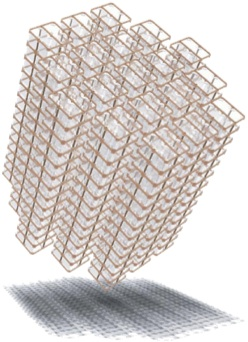
\includegraphics[width=0.225\columnwidth]{towers.jpg} 
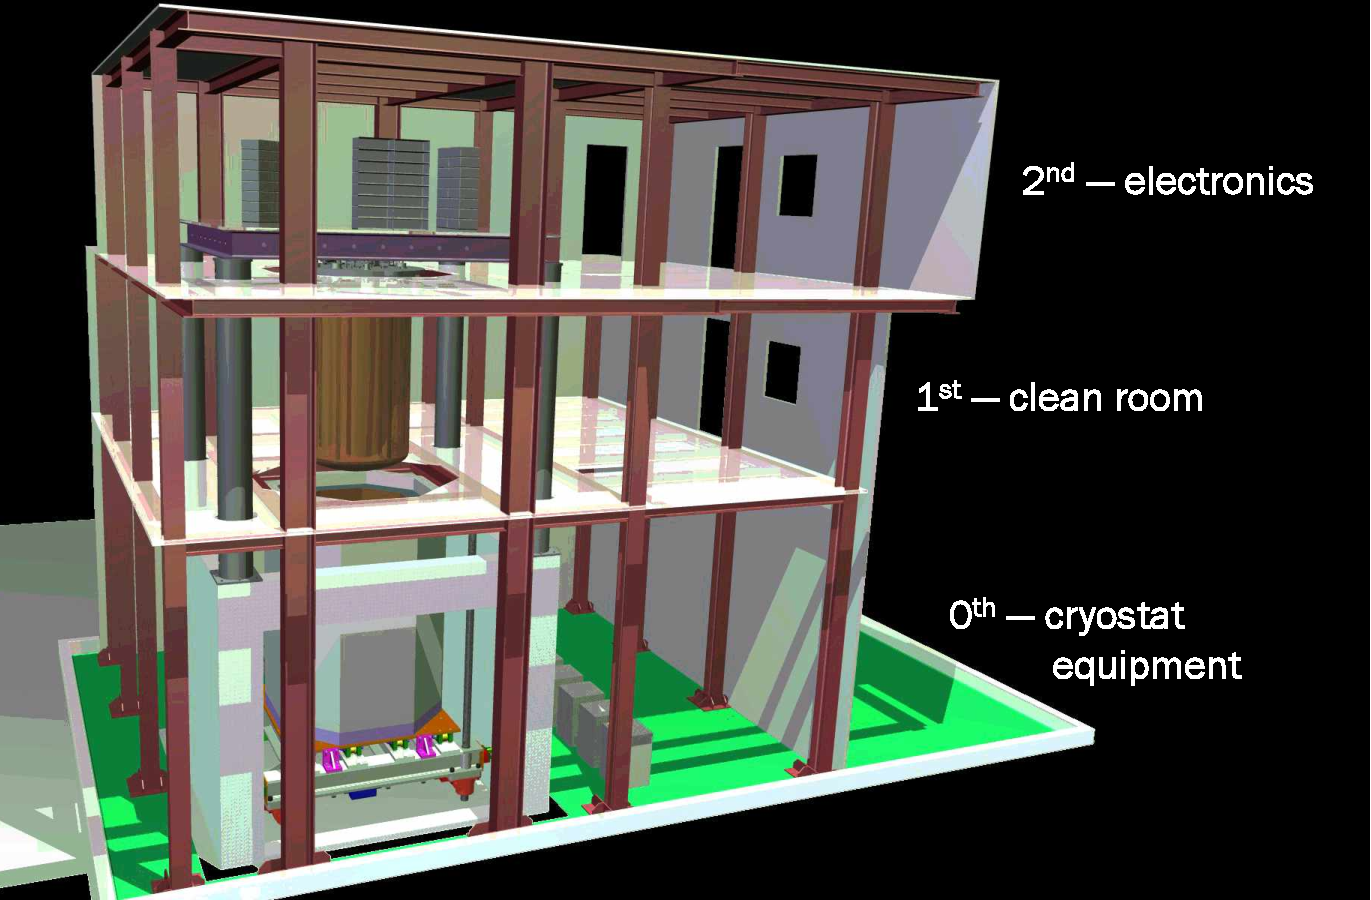
\includegraphics[width=0.505\columnwidth]{CUORE-hut-cross-section-labeled.pdf} 
\end{center}
\caption{\label{layoutCuore} The CUORE detector: the arrangement of the crystals into 19 towers (left) and the layout the CUORE detector in its clean hut (right).  }
\end{figure}

The CUORE experiment is searching for \zeronu~in $^{130}$Te with an endpoint of 2.527~MeV. Examining the terms in Eq.~\ref{sens0nu}, the advantages of this isotope and technology become obvious. The natural abundance is 33.8\% which means isotopic enrichment is not necessary. The only the gamma ray from the U/Th chains above the endpoint energy is the 2.6~MeV gamma ray from the decay of $^{208}$Tl.  The detector is constructed out of crystals of TeO$_{2}$  operated at 10~mK as bolometers. The CUORE crystals have achieved energy resolutions of 1.5~keV at the endpoint energy. This is on a par with all but the best germanium detectors. 

The performance of these crystals is the result of a 30-year program of experiments searching for \zeronu~with TeO$_{2}$ bolometers first proposed by Fiorini and Niinikoski  in 1984\cite{Fiorini198483}. It is the background levels which benefit most from this vast experience in crystal growth, mechanical support, readout, and handling, in addition to expertise in cryostat construction. The immediate predecessor of CUORE is the CUORICINO experiment, which ran from 2003-2008.  CUORICINO achieved a background level of 0.15 counts/(keV kg yr) in one tower of crystals representing 11.3~kg of isotope. They were able to set a limit of $T_{1/2}^{0\nu} > 2.8\times10^{24}$yrs at the 90\% C.L.

In order to improve upon this limit, the mass of the detector will be increased to 741~kg, representing  206 kg of isotope. The crystal dimensions are 5$\times$5$\times$5~cm$^{3}$ and they will be arranged into 19 towers as shown in Fig.~\ref{layoutCuore} (left). This factor of 20 increase in size is complemented by a factor of 20 reduction in the background levels through better choices of materials for the cryostat and mechanical supports, and better crystals handling. The first indications of success in background reduction are coming in now as the first data from CUORE-0 is analyzed by the collaboration. CUORE-0 is the first production tower of crystals for CUORE operated in the CUORICINO cryostat. A preliminary analysis presented at TAUP2013, the background level is 0.074$\pm$0.012 counts/(keV kg yr) , a factor of 2 reduction from the CUOROCINO background level of 0.153$\pm$ 0.006 counts/(keV kg yr).  With backgrounds on the order of 0.05 counts/(keV kg yr), CUORE-0 will be sensitive to $\langle m_{\beta\beta} \rangle$ between 0.17-0.39~eV. This is comparable to the current limits from EXO 0.14-0.38~eV\cite{EXO2012}, KamLAND-Zen combined with EXO 0.12-0.50~eV\cite{KZ0nu}, and GERDA 0.2-0.4~eV\cite{gerda2013}.  The full CUORE detector should then push down to 0.041-0.095~eV and begin to explore the inverted hierarchy.

As CUORE-0 runs, the rest of the towers are being constructed, and they will be installed by the end of 2014. The crystals are read out using Neutron Transmutation Doped (NTD) Ge thermistors. The assembly is labor-intensive, and one reason is that the NTDs are glued to each crystal individually. Therefore, all collaborators will be needed to help in this effort and in shift taking on CUORE-0. In parallel, the cryostat will be commissioned and integrated with the calibration system. The final configuration of the front-end electronics is being finalized now and everything is on schedule for data taking and first results from the full CUORE in 2015.

\subsection{Commissioning and Analysis Manpower}

The preliminary CUORE-0  analysis presented at TAUP2013 was a valuable exercise not only because it provided the first confirmation that the crystal handling procedures were achieving the desired background levels, but because it also tested the available manpower for the CUORE commissioning and analysis.  The analysis was performed by the equivalent of 2.5 postdocs and two graduate students: Jon Ouellet on data quality and Brian Zhu on MC background analysis. This was a combined U.S. and Italian analysis. Compared to similar experiments with multiple analysis teams and looking to the future with the the jump to almost 1000 channels, we are critically understaffed.  There has been a large U.S. investment in the construction of CUORE and we need to ensure that we have the manpower to extract all the excellent physics that can come from this multipurpose detector.

The MC is a self-contained task that exemplifies the current issues.  The full CUORE MC is an extension of the CUORICINO MC. The advantage is that much of the physics has been verified, and geometry has been implemented, however the output is a simple text file of energy deposition and crystal number. This is both an infrastructure issue since with the bigger detector and higher statistics the text file will become unweildly.  This is also an issue for the sophistication of the analysis. Much more information can be extracted from the MC, but a more complex output format, usually ROOT-based,  is needed to capture this information. More manpower is needed to implement upgrades to the MC and do the MC data background verification. The postdoc supported by this grant will take on the leadership for this task.

The other measure of the 
\begin{table}
\footnotesize
\begin{center}
\begin{tabular}{ l l l l l}
\hline
Student & Institution & Analysis & Graduation & Funding \\
\hline
Jon Ouellet & UC Berkeley & \zeronu~CUORE0 & 2015 & Yes \\
Brian Zhu  & UCLA & \zeronu~CUORE0 & 2015 &  1 year  \\
Nick Chott  & USC & Axion via Primakoff  conversion & 2018 & Yes \\
Nelson Camilo Posada-Aquirre  & USC & Axion via axio-electric effect  & 2018 & Yes \\
Alexey Drobizhev & UC Berkeley & \zeronu~CUORE & 2018 & Yes \\
Jeremy Cushman  & Yale &  \zeronu~CUORE & 2017 & Yes \\
Erin Hansen & UCLA & Majoron Decay CUORE & 2019 & {\bf This Proposal} \\
\hline
\end{tabular}
\caption{\label{studentManPower} Summary of U.S. students working on CUORE}
\end{center}
\end{table}


\section{Research Plan}

\subsection{Previous Experience}
%~1 page.
The KamLAND experiment is a reactor antineutrino experiment. It uses the sum of Japan's nuclear reactors as its neutrino source, and has an average baseline of $\sim$200~km, the distance to the Kamioka mine that houses the 1~kton of liquid scintillator that is KamLAND. Nuclear reactors produce a spectrum of antineutrinos that extends up to $\sim$8.5~MeV. Given this energy range and baseline, KamLAND is perfectly situated to measure neutrino oscillations with a $\Delta m^{2}_{21}\simeq10^{-4}$eV$^{2}$ as the oscillation is observable across the spectrum, as shown in Fig.~\ref{kamPlot}\cite{Eguchi:2002dm, Araki:2004mb,Abe:2008aa}. The current best measurement from KamLAND is $\Delta m^{2}_{21}=7.50\pm0.2\times10^{-5}$eV$^{2}$ with $\tan^{2}_{12}=0.492_{-0.067}^{+0.086}$\cite{Gando:2010aa}. The addition of constraints from solar experiments reduces the uncertainty on the mixing angle, but not the $\Delta m^{2}$,  giving $\Delta m^{2}_{21}=7.50_{-0.20}^{+0.19}\times10^{-5}$eV$^{2}$ with $\tan^{2}_{12}=0.436_{-0.030}^{+0.036}$.

%The wrap figure is a pain. Let's start with plain figures and add the wrap figures as needed.
%\begin{wrapfigure}{l}{0.35\textwidth}
%\begin{center}
%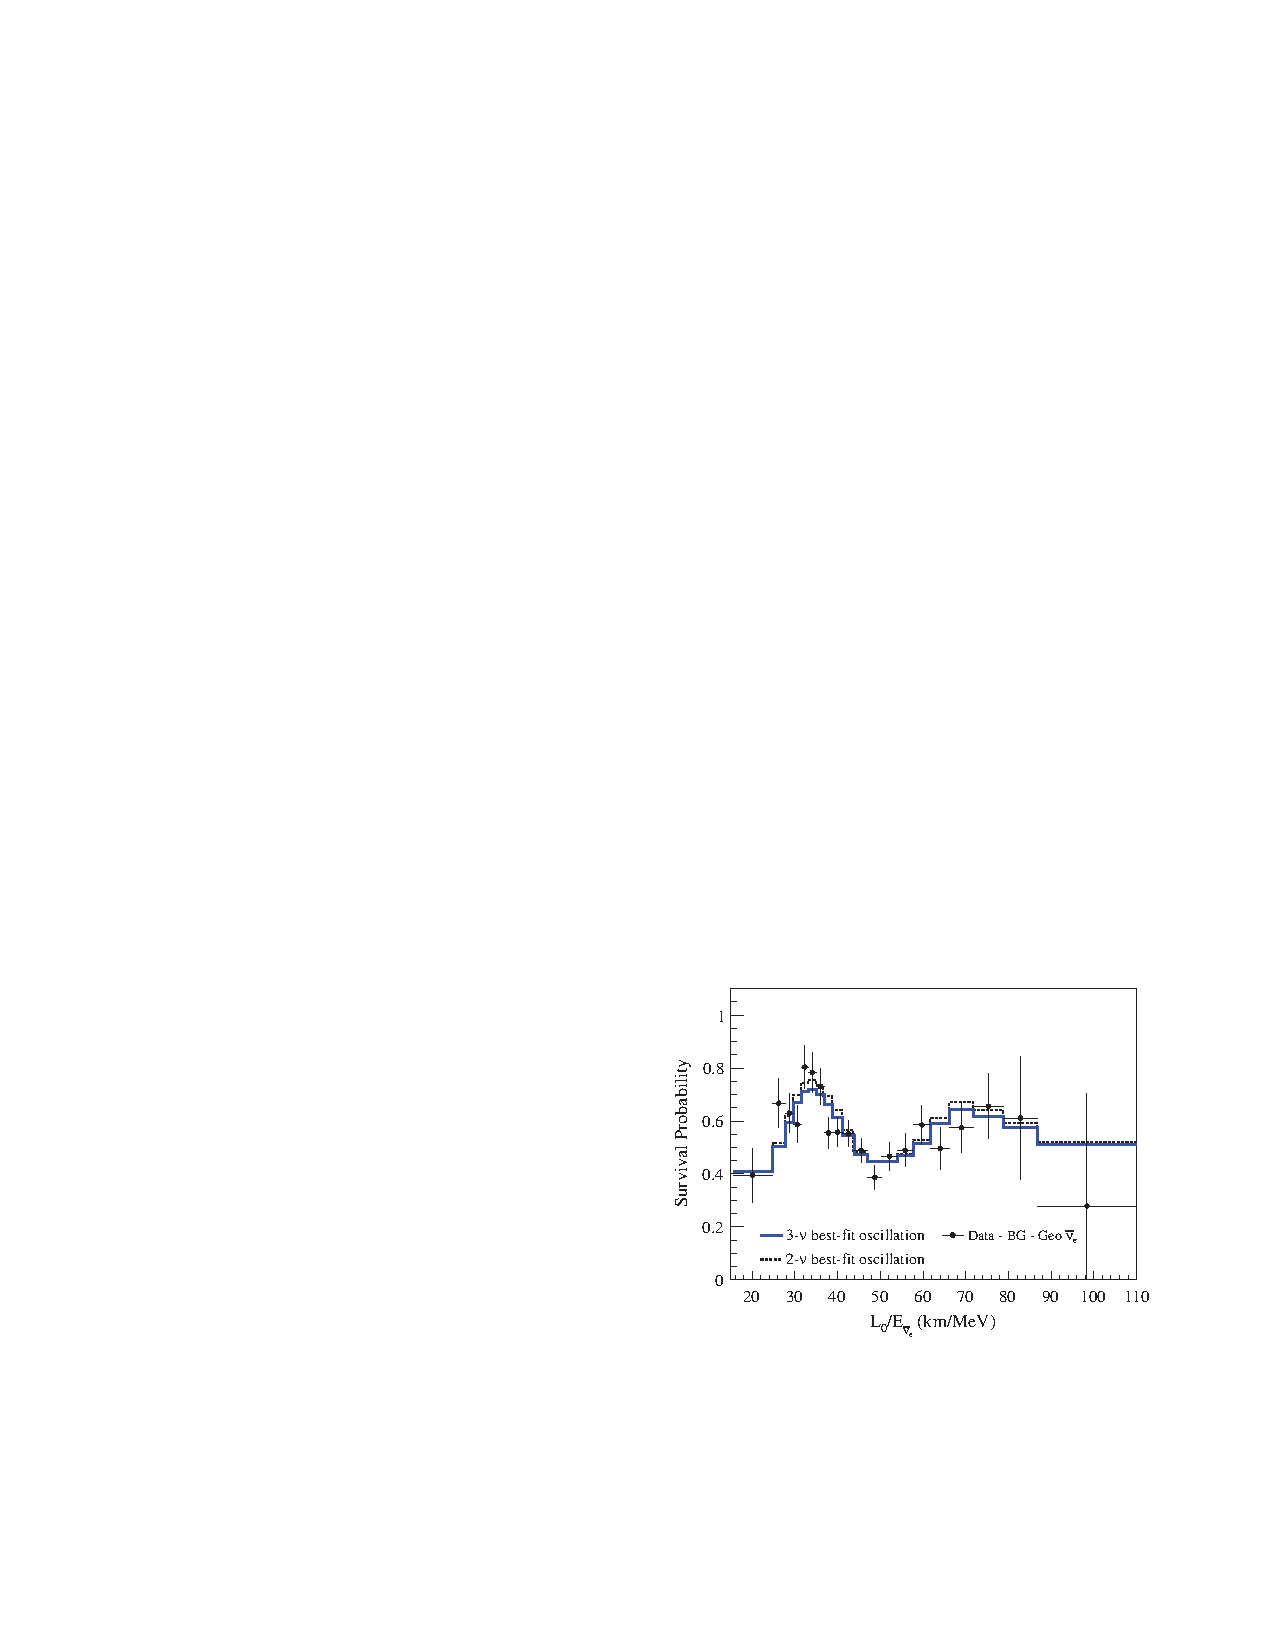
\includegraphics[width=0.30\columnwidth]{KamLAND_Osc_Plot.pdf} 
%\end{center}
%\caption{{\footnotesize \label{kamPlot} Typical absorption and emission spectra for quantum dots.}}
%\end{wrapfigure}
%FIXME: reduce size and trim.
\begin{figure}
\begin{center}
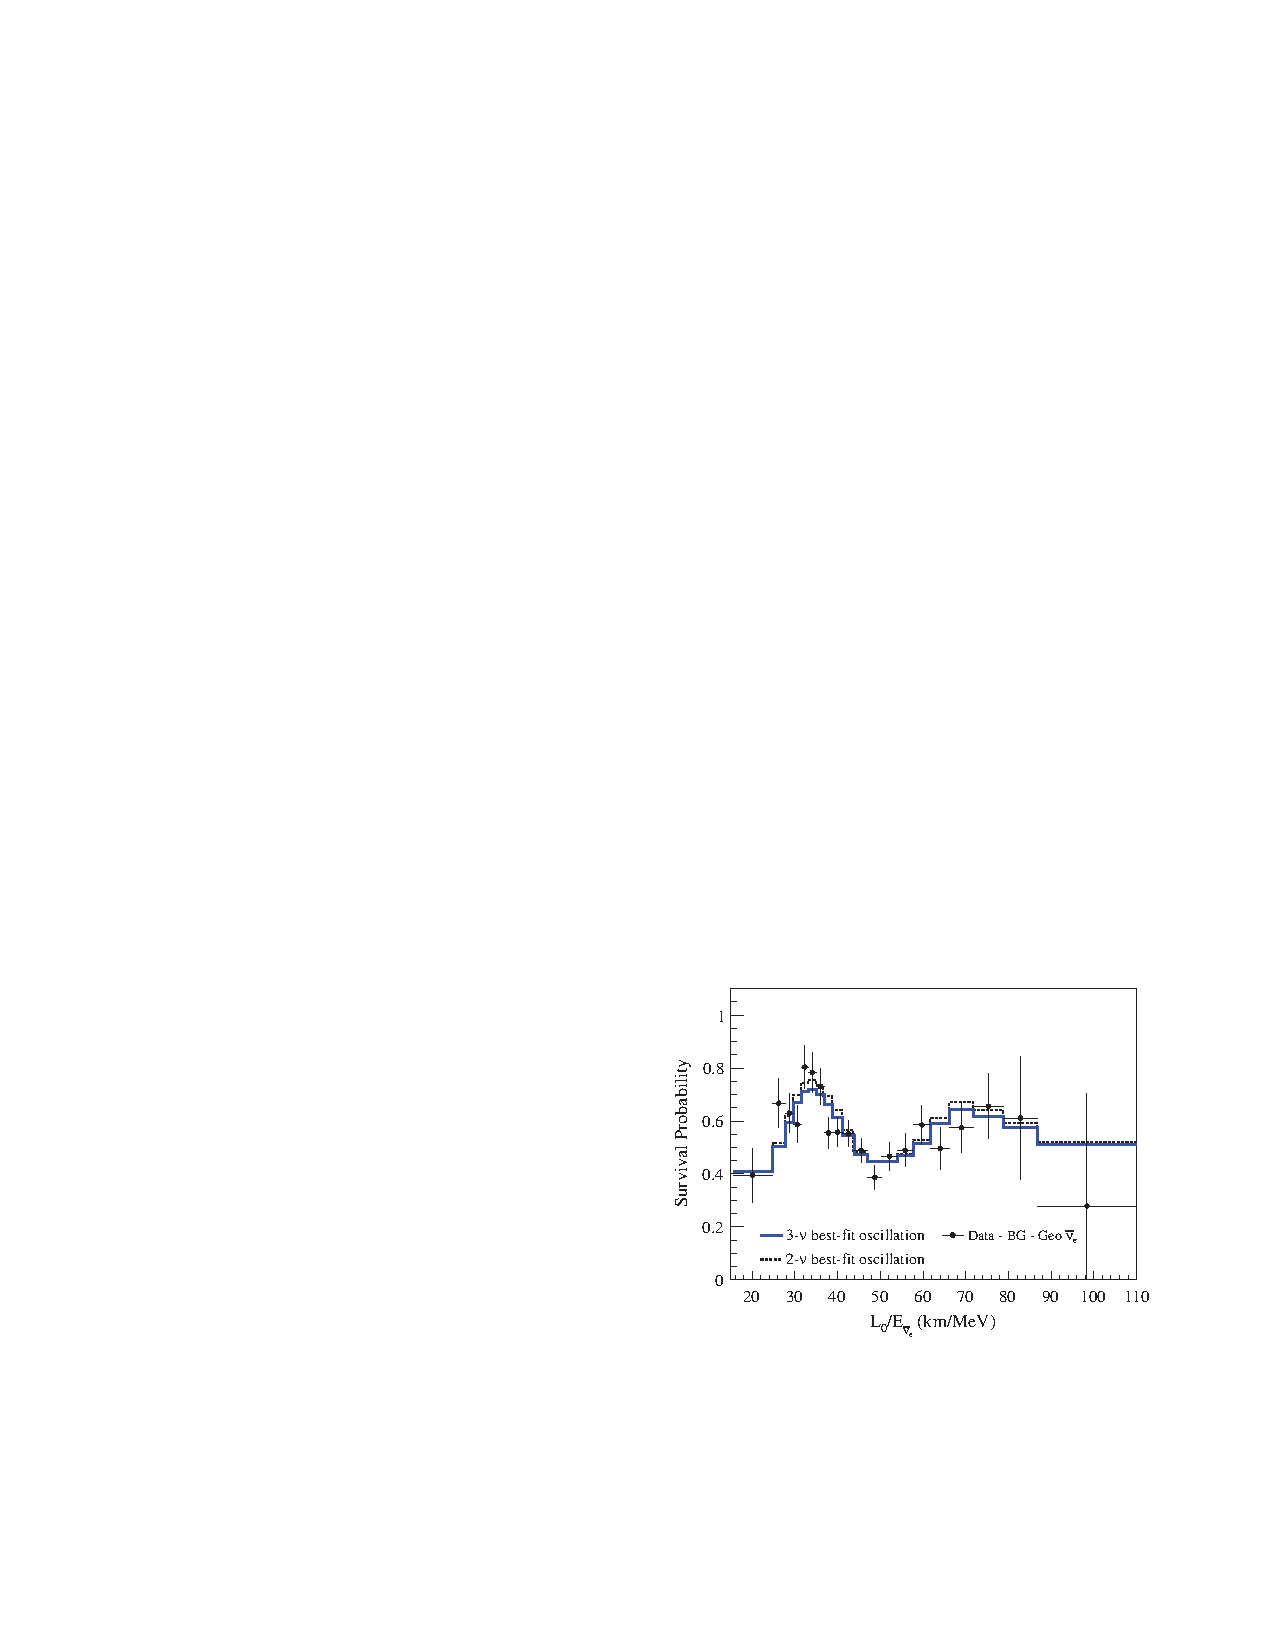
\includegraphics[trim=0.3cm 0.1cm 0.5cm 0.1cm, clip=true, width=0.58\columnwidth]{KamLAND_Osc_Plot.pdf} 
\caption{\label{kamPlot} The observed KamLAND antineutrino spectrum plotted as a function of L/E is shown for the most recent data set \cite{Gando:2010aa}.}
\end{center}
\end{figure}

It is the physics of the matter effect in solar neutrinos which makes those experiments more sensitive to the mixing angle $\theta_{12}$.  In KamLAND matter effects are small, it is the reactor systematics uncertainties in the reactor flux prediction that dominate the sensitivity to $\theta_{12}$. This was not the case in the first  publications\cite{Eguchi:2002dm, Araki:2004mb}.  A full-volume calibration system allowed radioactive sources to be deployed throughout the fiducial volume\cite{fourpi}. This reduced the uncertainty in the fiducial volume and confirmed the understanding of the energy scale, the key systematic uncertainty in the $\Delta m^{2}_{21}$ measurement.  

The PI worked on the instrumentation packages that were used in the calibration system. The packages consisted of pressure sensors, temperature probes, and accelerometers. The readout was made difficult due to the requirement that the signals go through a slip-ring to allow the system's cables to turn. There was also significant noise generated by the system's motors. This hampered the use of the packages to position the system. We were, however, able to extract a beautiful temperature map of the detector, which greatly helped our understanding of convection in the detector. This was particularly important during the scintillator purification effort that followed the deployment of the full-volume calibration system. The instrumentation packages wrote their data directly to a database; this proved useful for later analysis.

The system was inserted right before the start of the scintillator purification effort. Consequently, the requirements to prevent U/Th contamination due to the system were quite stringent. The PI was responsible for the cleaning and certification of the system components. The protocol was developed in close collaboration with colleagues who were also taking part in the EXO experiment; thus the protocol developed for that experiment \cite{Leonard:2007uv} follow closely the one for KamLAND\cite{fourpi}. These efforts proved successful, and a deployment of the system at the end of the low-background phase of KamLAND in June 2010 showed limited contamination resulting from the insertion of the system.  Ultimately, the techniques developed for cleaning and counting components of this system are general to low-background experiments from dark matter to double-beta decay; therefore this experience carries over nicely to CUORE.

\begin{figure}
\begin{center}
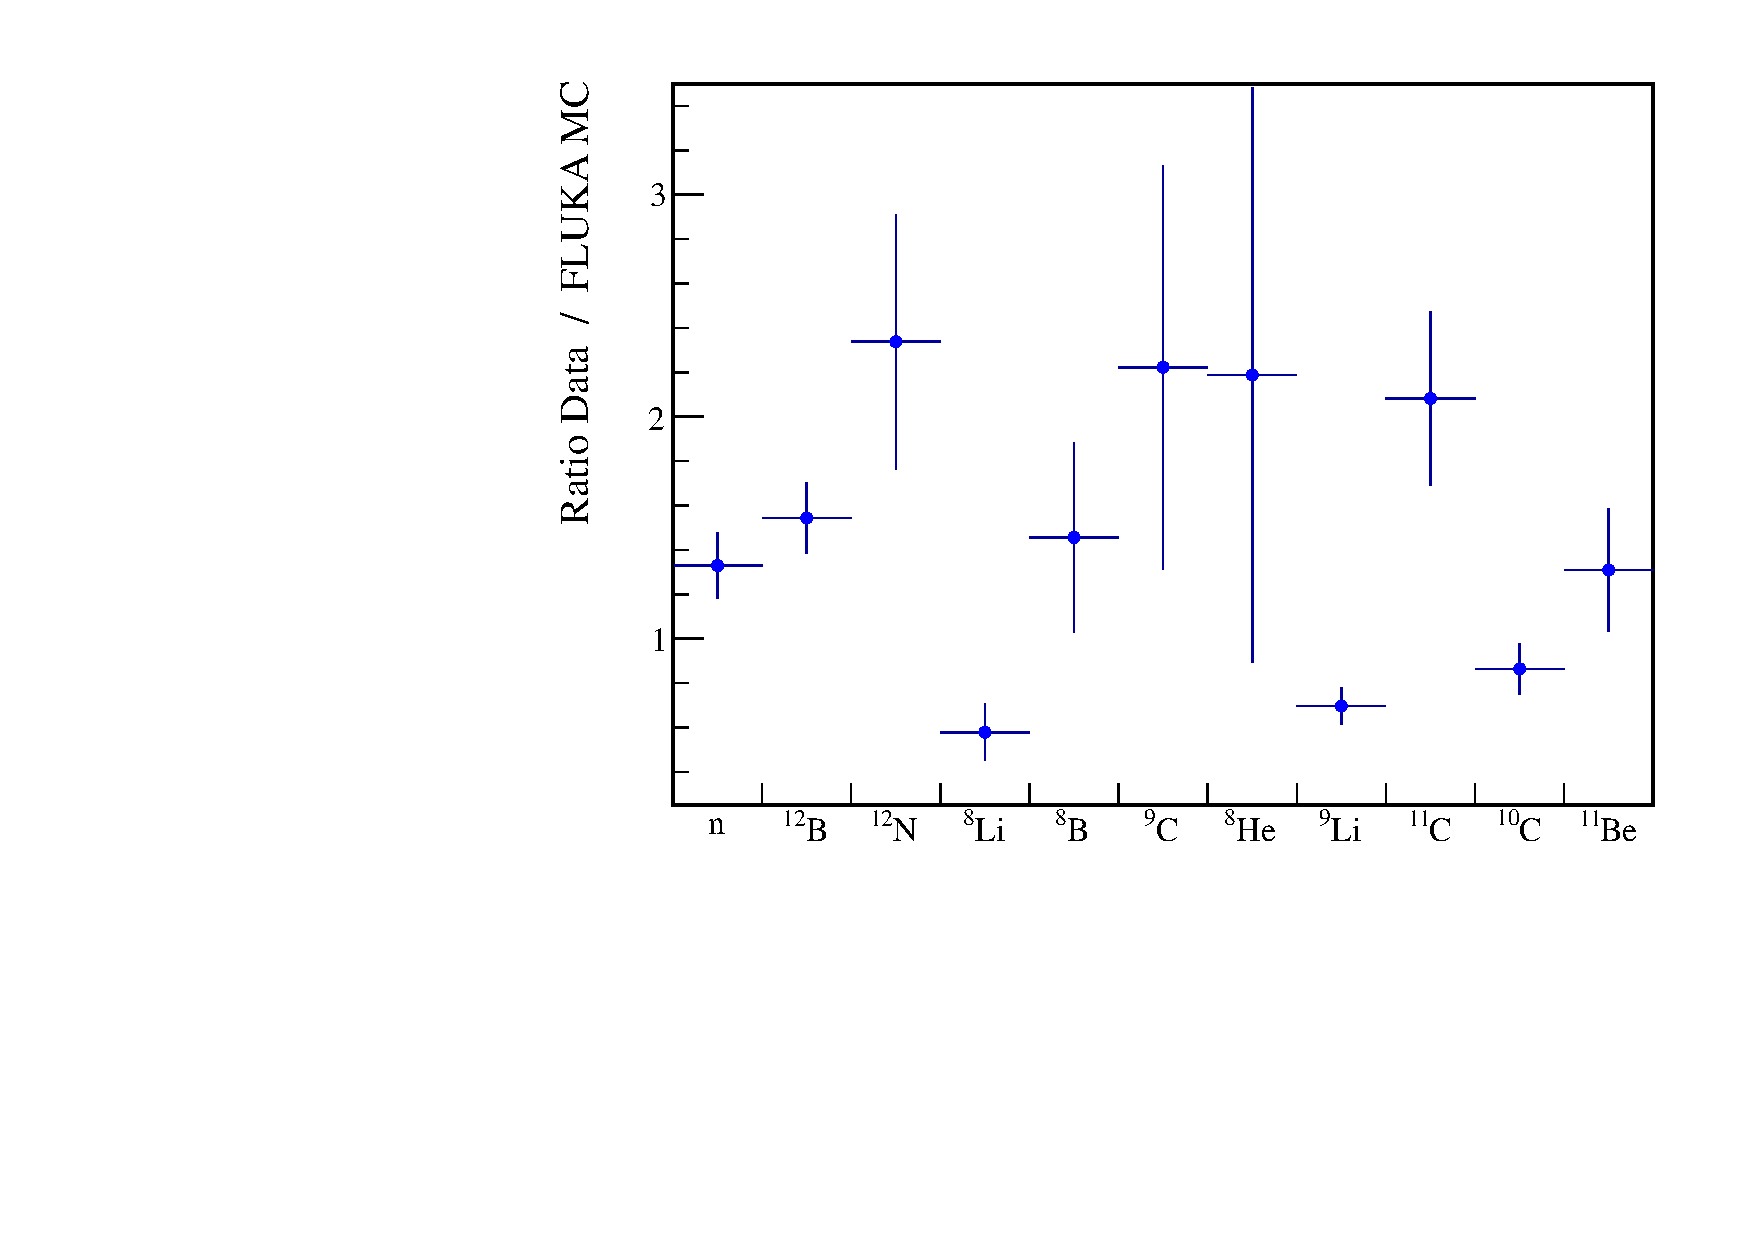
\includegraphics[width=0.48\columnwidth]{kamlandspall.pdf} 
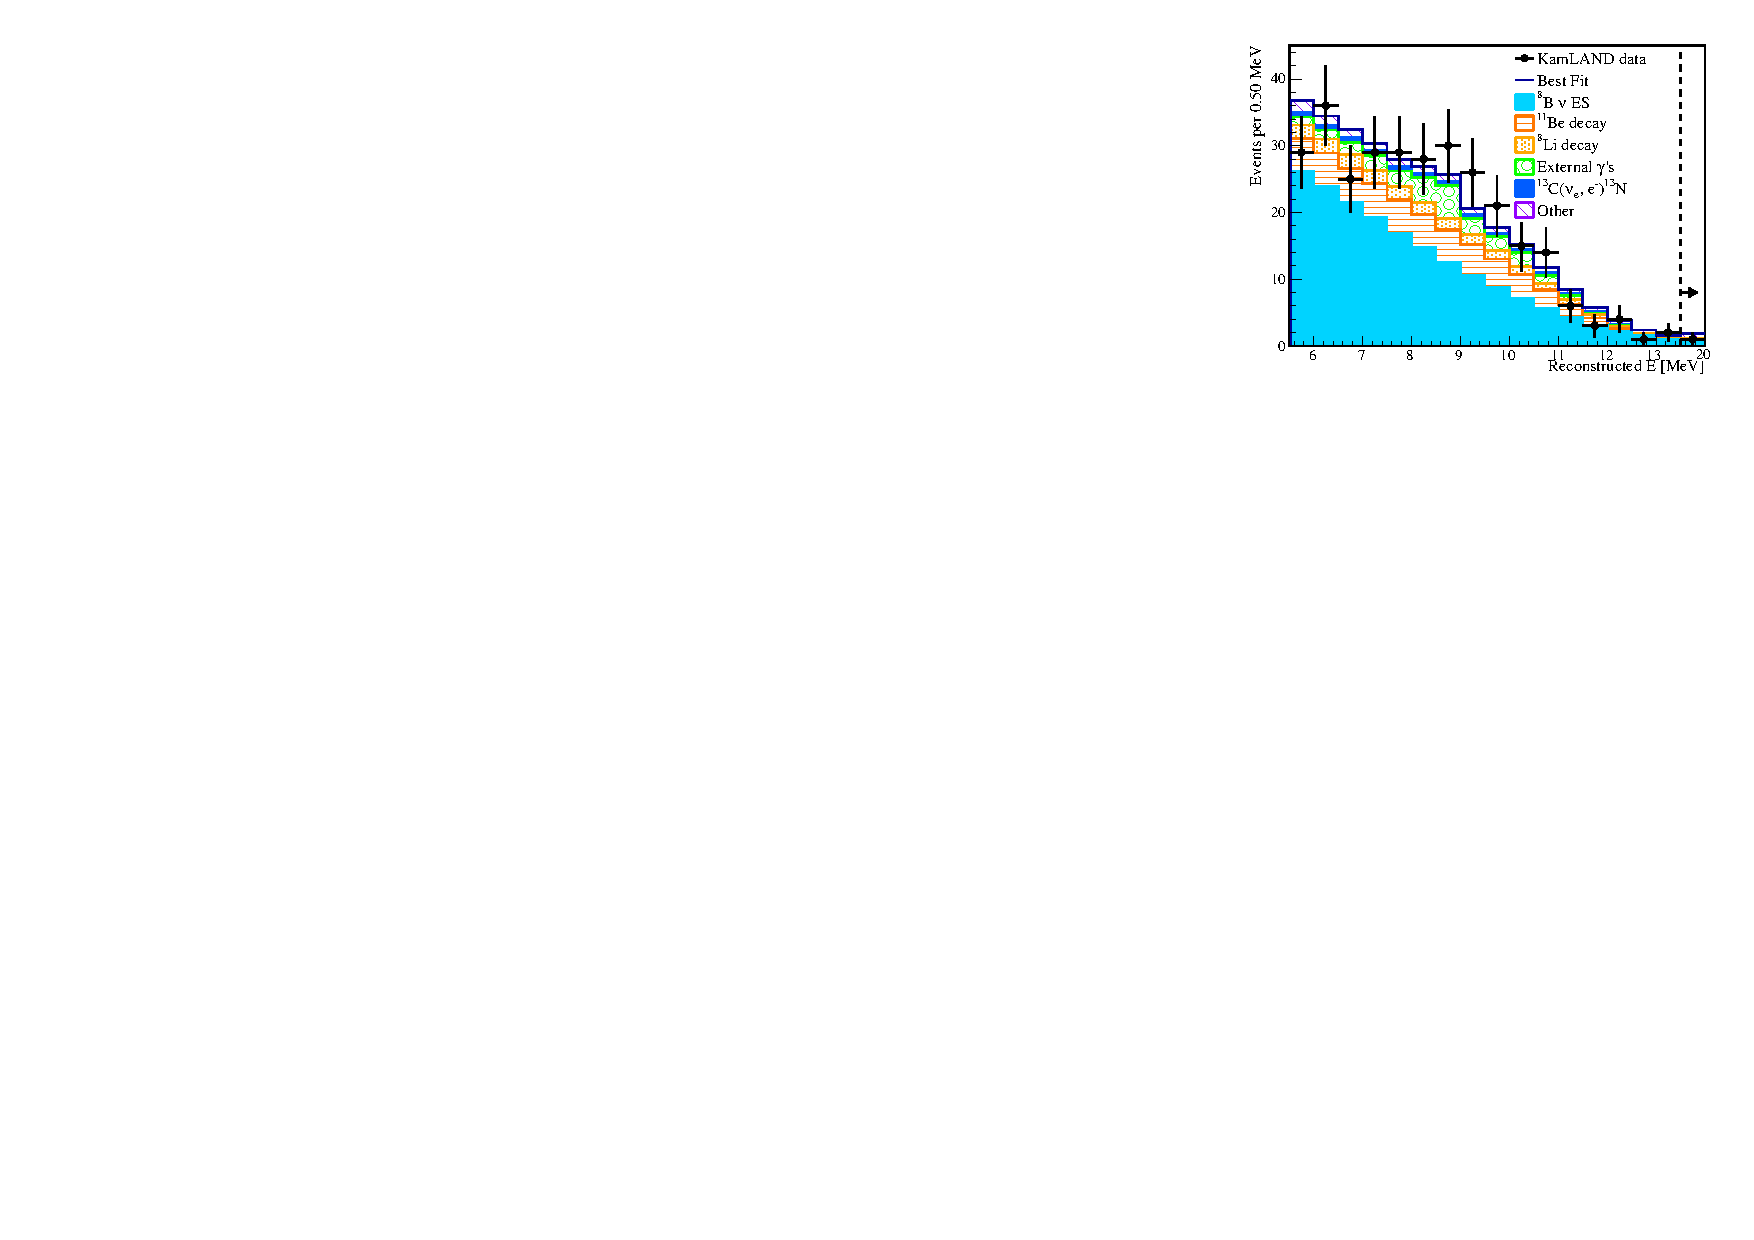
\includegraphics[width=0.48\columnwidth]{Kam8BSpec_1Sept2011.pdf} 
\caption{\label{kamSpallSol} The measured isotope production by muons in KamLAND scintillator compared to the FLUKA simulation\cite{kamspall} (Left). The fit to the spectrum of single events above 5.5~MeV to extract the $^{8}$B solar neutrino event rate \cite{kamboron}(Right). The solar neutrino analyses rely heavily on the muon spallation analyses, as do the subsequent KamLAND-Zen measurements.}
\end{center}
\end{figure}

KamLAND detects antineutrinos using inverse beta decay, which provides a coincidence signal between the prompt positron annihilation and the delayed neutron capture. The coincidence effectively removes backgrounds due to  radioactivity from the U/Th chains and muon spallation. The main remaining backgrounds are from accidental coincidences made between U/Th radioactivity and external neutrons, and the $\beta$-n decays of $^{9}$Li and $^{8}$He.  KamLAND can also be used to detect solar neutrinos. The neutrino-electron elastic scattering signal is the recoil of a single electron. This single signal is more difficult to extract because the decays of all the daughters of the U/Th chains, and the beta decays of muon spallation products are backgrounds. 

The $^{8}$B solar neutrino analysis on KamLAND was led by the PI. The threshold of the analysis is set by the endpoint of the $^{208}$Tl spectrum at a reconstructed energy of 5.5~MeV. The main background is the spallation product $^{11}$Be with an 11.5~MeV endpoint and a 13.8~s half-life. This background spawned a detailed study of muon spallation in KamLAND, including a Monte Carlo (MC) simulation of the production\cite{kamspall}. Spallation backgrounds are ubiquitous to low-background experiments, and these results expanded the data points used for benchmarking simulation beyond neutrons for the first time. On average, FLUKA underestimates the production; however, it is interesting to note that some isotopes are underproduced in Fig.~\ref{kamSpallSol}. In the future, it would be nice to compare these results to those from Borexino and SNO+.

The $^{8}$B neutrino flux measured by KamLAND is 2.77$\pm$0.26(stat)$\pm$0.32(syst)$\times10^{6}$cm$^{-2}$s$^{-1}$\cite{kamboron}. This result is in good agreement with the very precise Super-Kamiokande measurements\cite{skboron}, and those from SNO\cite{snoboron} and Borexino\cite{borexinoboron}. The Borexino analysis uses the KamLAND spallation results to quantify their background.  The spallation analysis is also key to understanding the backgrounds from $^{11}$C in KamLAND-Zen's \isoxe~double-beta decay analysis\cite{KZ2nu}. Finally, the relative production of the $\beta$-n isotopes $^{9}$Li versus $^{8}$He has been used in the analyses for $\theta_{13}$ by the Daya Bay\cite{dayabay}, RENO\cite{reno}, and Double Chooz\cite{dcone, dctwo} experiments.

\subsection{Double Chooz Experience} 
%~1 page.
The Double Chooz experiment, like KamLAND, uses nuclear reactors as a source of antineutrinos and inverse beta decay to detect them. Unlike KamLAND, it is positioned only 1~km  from the two Chooz cores, making it sensitive to the effect of the mixing angle $\theta_{13}$. To enhance the inverse beta decay signal, a Gd-doped scintillator is used as the target. The PI had three leadership roles on the experiment: slow monitoring leader, data production leader, and analysis coordinator for the predominantly U.S.-based analysis cluster, Cluster United (CU). 

The slow monitoring hardware consists of several different instrumentation packages spread throughout the experiment.  Packages to monitor temperature and magnetic fields are deployed among the PMTs in the main detector. Temperature monitoring is deployed in the other detector volumes and throughout the hall. The experimental hall is also instrumented with humidity and radon monitors. Finally, daughter boards are used to monitor the input voltages on the front-end electronics cards. A netbook computer running Debian Linux is used to read out the hardware. This proved to be a practical and frugal choice, since a netbook is designed to run from both a battery and wall power and has a small footprint. In addition, devices such as remotely controlled power strips from other groups are integrated into the system. 

All data is written to a MySQL database with a uniform format that allows easy access and analysis from both a web interface and the ROOT software package. The trickiest devices to integrate were those operated by LabVIEW. In the end, we used a script to parse the LabVIEW data and write it to the database. Those watching the detector monitor the most critical data in real time using the greater Double Chooz Online system. This is a JAVA-based software package which provides plots and sends error messages to the shifter. 

As the slow monitoring leader, the PI  ended up gaining responsibilities in many different areas of detector construction and operation.  These ranged from the configuration and maintenance of the experiment's MySQL server to organizing tools for remote operation and shift taking. The most critical part of this work was the delicate task of filling the detector. Temperature fluctuations are a danger to the mechanical integrity of the detector and to the systematic uncertainty on how many protons are in the target volume. The PI was an expert on the filling system and continued to use the slow monitor data to understand the uncertainties in the analysis.

In addition to the slow monitoring, the PI ended up leading the data processing production. This grew out of the PI's work with the database. Tools were developed with MIT graduate student Kazuhiro Terao for file tracking and data quality determination. This evolved into responsibility for all data processing, from raw data transferred from Chooz to reduced event trees for high-level analyses. Due to the PI's strong involvement in the reactor flux prediction, this also grew to include the production of the official reactor antineutrino and $^{9}$Li MC; the other backgrounds are extracted purely from data.

The PI strong involvement in the reactor simulation is the result of Double Chooz's two-phased data taking approach. Currently the experiment is finishing the first far-detector-only phase; therefore, a full reactor simulation is needed to predict the flux of neutrinos in the far detector. The PI worked closely with MIT graduate student Chris Jones who generated this prediction using the DRAGON code\cite{DRAGON1994}. The code simulates the individual fuel components which make up the reactor core, and directly solves the neutron transport equation. This is in comparison to the main code, MURE\cite{MURECode,Meplan2005} , which models the full reactor core and uses MC techniques to solve the neutron transport equation. The PI led an effort to benchmark these codes against the chemical analysis of fuel from the Takahama reactor in Japan and the results of other codes\cite{takahama}. The Takahama data is a standard data set to benchmark reactor codes against. In the past, little care had been taken to understand its systematic uncertainties. In this work, we consulted the original authors, evaluated the systematic uncertainties, and propagated them to the fission rates. This work is useful to the neutrino community at large as DRAGON is a fast, free, open-source code and reactors are a useful source of antineutrinos for other studies. DRAGON is already being used outside of Double Chooz by the Daya Bay collaboration in their studies of systematic uncertainties\cite{dayabay}.

As the CU analysis coordinator, it was the PI's close connection to the reactor group and experience from KamLAND that led CU's analysis to become the analysis used in the first publication\cite{dcone}, and laid the groundwork for the improvements in the second analysis\cite{dctwo}. The power of the KamLAND analysis comes from using rate and energy or shape information to extract the oscillation parameters because the main backgrounds, $^{9}$Li and fast neutrons, extend to higher energies. This requires better understanding of the energy scale of the detector and the shape of the antineutrino spectrum. Motivated by this experience, the PI started work more than a year before data taking began, and had University of Alabama graduate student Igor Ostrovskiy and Columbia University graduate student Arthur Franke visit  MIT to start putting together CUfits, the CU package for extracting $\theta_{13}$ using a rate plus shape fit.

Due to time constraints for the first analysis, the original plan of a full Multisim treatment to propagate low-level uncertainties in the MC light model to the energy scale was postponed, and an empirical correction derived from calibration data was used to correct discrepancies between the MC and data. This correction was verified using maps of detector response derived from isotropic spallation neutrons made by the PI. Similar maps are now used in the second analysis to reduce anisotropies in the data and MC. 

Thus, the main improvements between the first and second analyses come from the improvements in the background uncertainties and the energy scale. The significance of the disappearance is now at 2.9$\sigma$ with $\sin^2 2{\theta}_{13} = 0.109 \pm 0.030$(stat)$\pm0.025$(syst). This analysis also includes some upgrades to the $^{9}$Li MC generator. This was originally the work of the PI and Boston University undergraduate Claire Thomas. The PI has continued the work with Muhammad Elnimir, a postdoc from the French institution Subatech. As $^{9}$Li is the largest background, the work on the spectrum shape continues to be important.

\subsection{Continuing Work}
%~1 page.
The PI's involvement in Double Chooz is coming to a close. This proposal only asks for travel funds in the first year of the award to complete the installation of the slow monitor devices in the near hall and to attend two collaboration meetings to finalize the publication of the last three papers that the PI is leading. These papers are the instrumentation paper on the slow monitor system, a paper detailing the $^{9}$Li generator and recommending measurements to improve the $^{9}$Li spectral uncertainty, and finally a measurement of \zeronu~in $^{160}$Gd. 

The current best limit for \zeronu~in $^{160}$Gd is $T_{1/2}^{0\nu} > 2.3(1.3)\times10^{21}$yrs at the 68\%(90\%) C.L. from a Gd$_2$SiO$_2$:Ce scintillating crystal with an exposure of 0.969 kg$\cdot$yrs\cite{Danevich2001}. This is a less-utilized \zeronu~candidate because of its 1.72~MeV endpoint. The more familiar candidates have endpoints above 2~MeV for two reasons. The first is that the predicted rate
\begin{equation}
\label{half0nu}
(T_{1/2}^{0\nu})^{-1} = G_{0\nu}(Q_{\beta\beta}, Z) | M_{0\nu}|^{2} \langle m_{\beta\beta} \rangle^{2}
\end{equation}
is suppressed due the phase space factor $ G_{0\nu}(Q_{\beta\beta}, Z)$, where $ | M_{0\nu}|^{2}$ is the nuclear matrix element and $\langle m_{\beta\beta} \rangle$ is the effective Majorana mass of the neutrino. An updated calculation of these phase space factors can be found in Ref.\cite{phasespace}. The second reason is that the lower endpoint leads to more backgrounds from the U/Th chain. Currently, the PI is working to simulate all of the components that make up the spectrum of single events, as shown in Fig.~\ref{dcSpec}. If the self-shielding in Double Chooz attenuates the backgrounds sufficiently, an improvement of the limit, due to the larger Double Chooz exposure of $>$1.6~kg$\cdot$year, is possible. This is the first time that single events have been studied in Double Chooz, and the analysis provides a nice verification of the energy scale used in the main antineutrino analysis.

\begin{figure}
\begin{center}
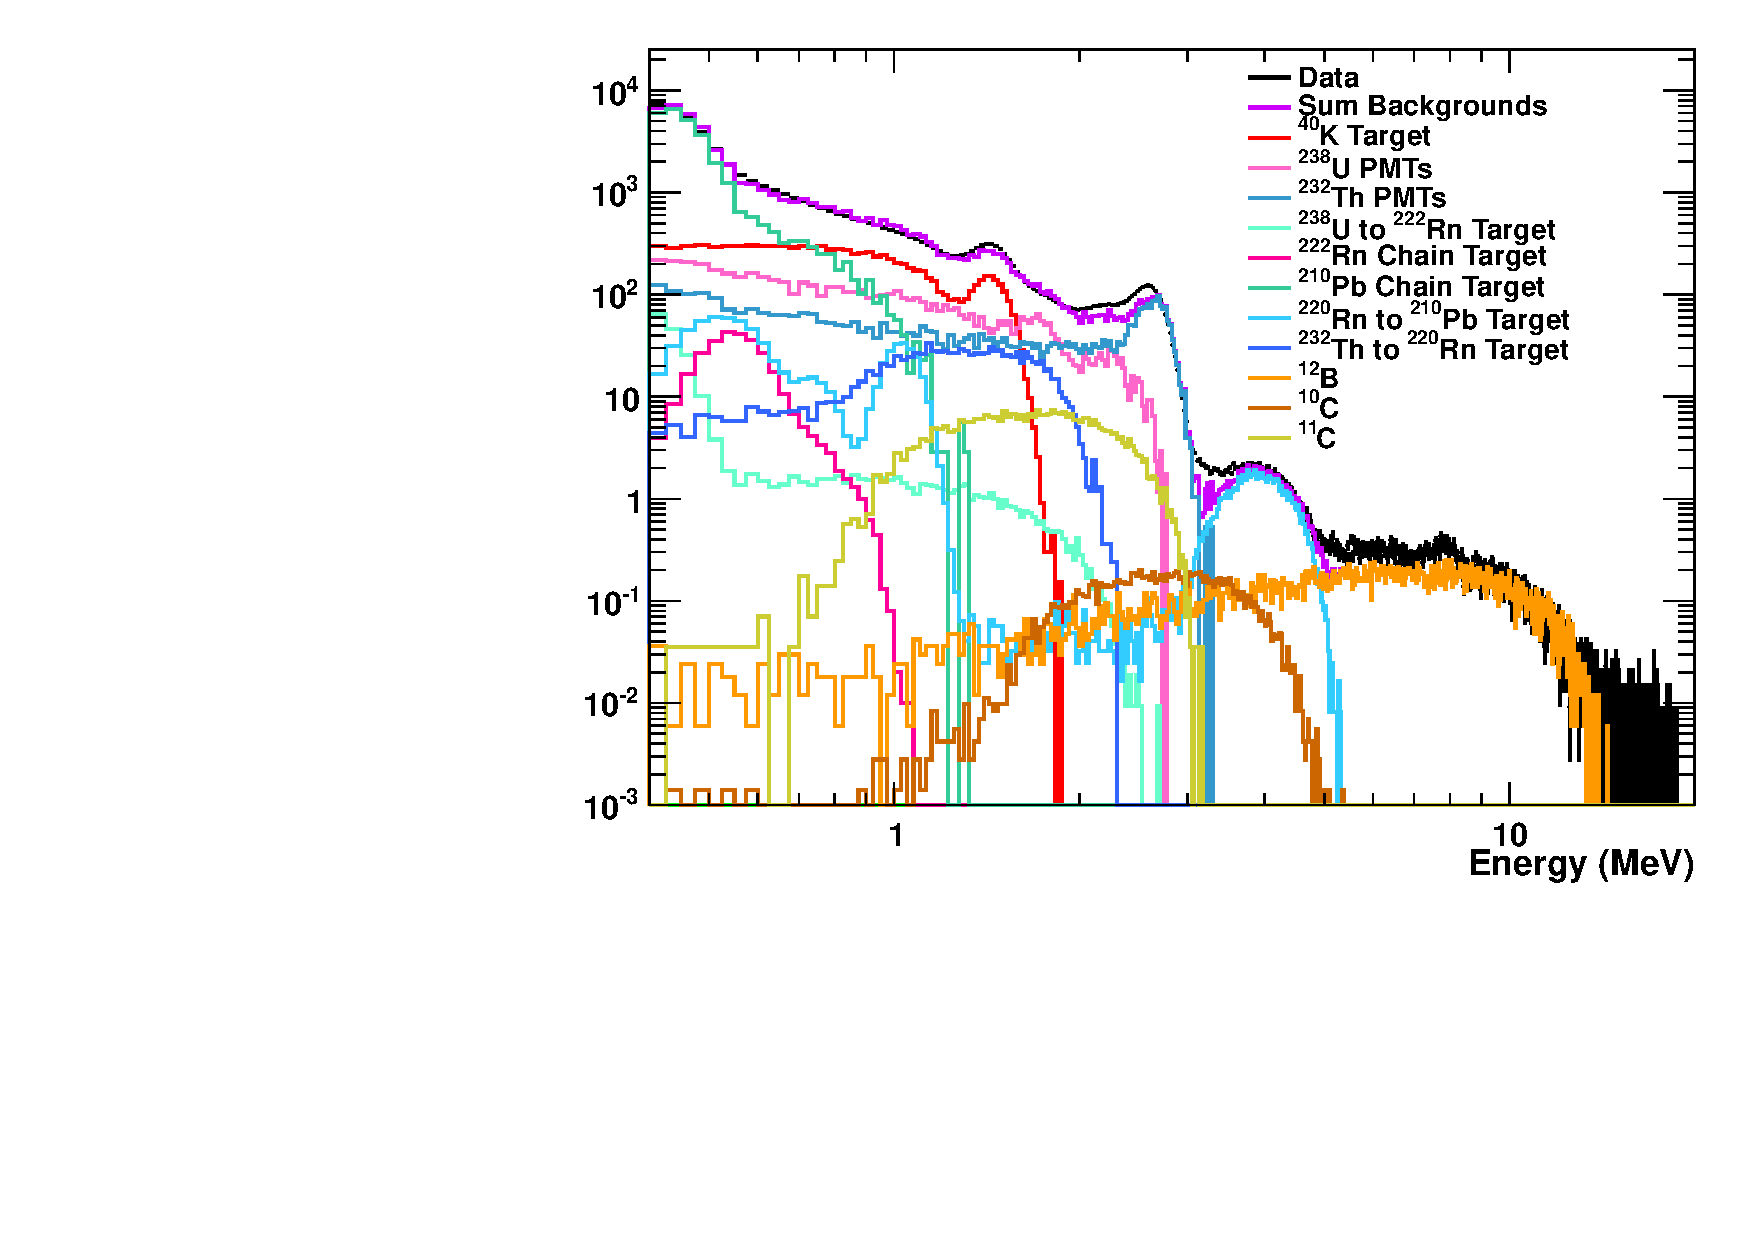
\includegraphics[width=0.58\columnwidth]{prettySpectrum_17July2012.pdf} 
\end{center}
\caption{\label{dcSpec} The spectrum of single events from a central region of the Double Chooz target of Gd-doped liquid scintillator. The fitting of the different components of the spectrum from the daughters of the U/Th chains internal and external to the liquid scintillator to muon spallation products is underway.}
\end{figure}

The analysis of \zeronu~in Double Chooz grew from the PI's interest in liquid scintillator detectors for  \zeronu~measurements. The final sensitivity of a \zeronu~experiment can be approximated as\cite{sens0nu}
\begin{equation}
\label{sens0nu}
T_{1/2}^{0\nu}(n_\sigma) = \frac{4.16\times 10^{26} yr}{n_\sigma} \left ( \frac{\epsilon a}{W} \right ) \sqrt{ \frac{Mt}{b\Delta(E)}}.
\end{equation}
In this approximation, $n_\sigma$ is the number of standard deviations for the resulting half-life, $\epsilon$ is the detector efficiency, a is the isotopic abundance, and W is the molecular weight of the source material. It is the next terms that truly distinguish experiments: M is the total mass of the source, t is the duration of the experiment, b is the background rate in the region of interest in counts/(keV kg yr), and $\Delta(E)$ is the energy resolution. The energy resolution is key in distinguishing signal from backgrounds, especially background from the standard model process two-neutrino double-beta decay  (\twonu).

It is the energy resolution that hinders liquid scintillator detectors like KamLAND-Zen compared to solid state detectors like CUORE; however, scaling up the mass of a liquid scintillator is straightforward. If more information like the direction of the outgoing electrons or simply better energy resolution could be achieved, then liquid-scintillator-based detectors may be a better option for the generation of experiments following CUORE. This is driving an R\&D effort to develop quantum-dot-doped liquid scintillator. Quantum dots are semiconducting nanocrystals made of cadmium, which has a candidate \zeronu~nucleus, $^{116}$Cd. Their unique optical properties, especially combined with new photodetection technology are already being explored for a multi-ton scale liquid scintillator experiment\cite{qdot}. 

The quantum dot work continues at UCLA thanks to equipment from the L'Or\'{e}al for Women in Science Fellowship and startup funds which support a postdoc who is an expert in metal-doped scintillators, Christoph Aberle. In this proposal, only travel funds to support the PI's continued involvement and development of future experiments at KamLAND are requested for these efforts; the main focus of this proposal is to support the PI's involvement in the CUORE experiment.

\section{Proposed Research Plan}
\subsection{CUORE:  The Search for Neutrinoless Double-Beta Decay}
\begin{figure}
\begin{center}
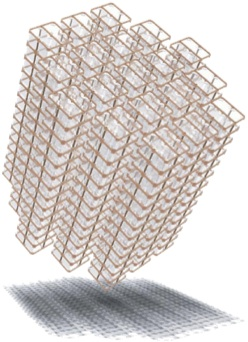
\includegraphics[width=0.225\columnwidth]{towers.jpg} 
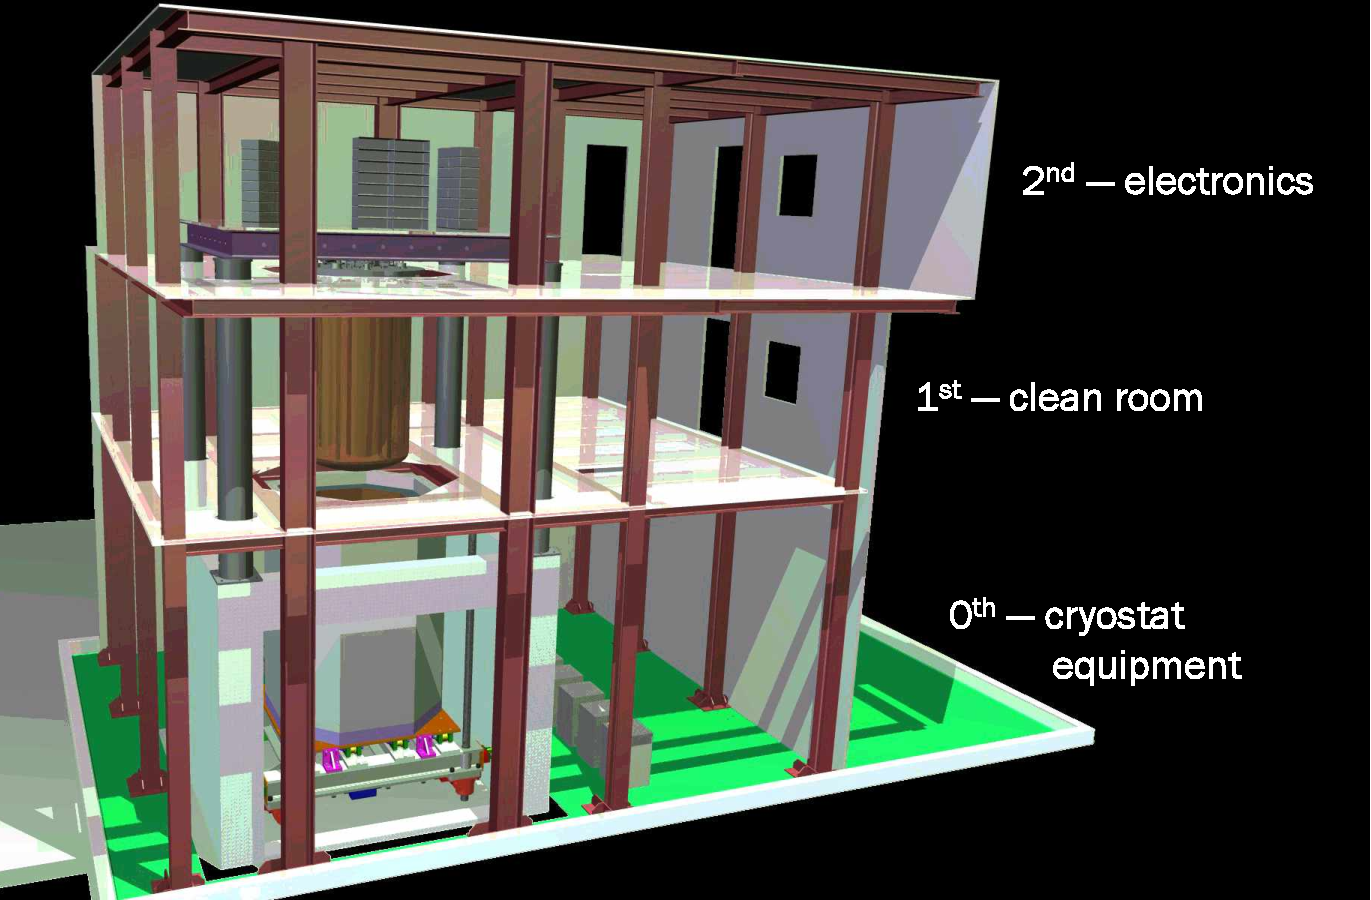
\includegraphics[width=0.505\columnwidth]{CUORE-hut-cross-section-labeled.pdf} 
\end{center}
\caption{\label{layoutCuore} The CUORE detector: the arrangement of the crystals into 19 towers (left) and the layout the CUORE detector in its clean hut (right).  }
\end{figure}

The CUORE experiment is searching for \zeronu~in $^{130}$Te with an endpoint of 2.527~MeV. Examining the terms in Eq.~\ref{sens0nu}, the advantages of this isotope and technology become obvious. The natural abundance is 33.8\% which means isotopic enrichment is not necessary. The only the gamma ray from the U/Th chains above the endpoint energy is the 2.6~MeV gamma ray from the decay of $^{208}$Tl.  The detector is constructed out of crystals of TeO$_{2}$  operated at 10~mK as bolometers. The CUORE crystals have achieved energy resolutions of 1.5~keV at the endpoint energy. This is on a par with all but the best germanium detectors. 

The performance of these crystals is the result of a 30-year program of experiments searching for \zeronu~with TeO$_{2}$ bolometers first proposed by Fiorini and Niinikoski  in 1984\cite{Fiorini198483}. It is the background levels which benefit most from this vast experience in crystal growth, mechanical support, readout, and handling, in addition to expertise in cryostat construction. The immediate predecessor of CUORE is the CUORICINO experiment, which ran from 2003-2008.  CUORICINO achieved a background level of 0.15 counts/(keV kg yr) in one tower of crystals representing 11.3~kg of isotope. They were able to set a limit of $T_{1/2}^{0\nu} > 2.8\times10^{24}$yrs at the 90\% C.L.

In order to improve upon this limit, the mass of the detector will be increased to 741~kg, representing  206 kg of isotope. The crystal dimensions are 5$\times$5$\times$5~cm$^{3}$ and they will be arranged into 19 towers as shown in Fig.~\ref{layoutCuore} (left). This factor of 20 increase in size is complemented by a factor of 20 reduction in the background levels through better choices of materials for the cryostat and mechanical supports, and better crystals handling. The first indications of success in background reduction are coming in now as the first data from CUORE-0 is analyzed by the collaboration. CUORE-0 is the first production tower of crystals for CUORE operated in the CUORICINO cryostat. It is expected to reach a background level of 0.05 counts/(keV kg yr) and improve the CUORICINO limit.

The sensitivity of \zeronu~searches are often plotted as a function of the lightest neutrino mass versus the effective Majorana mass of the neutrino, where Eq.~\ref{half0nu} is used to convert the measured half-life into the effective Majorana mass of the neutrino $\langle m_{\beta\beta} \rangle$. This means that uncertainties in the matrix element calculation lead to a range of sensitivities for $\langle m_{\beta\beta} \rangle$, indicated as a hatched region in Fig.~\ref{sensCUORE}. The green region represents a neutrino mass structure consistent with the inverted hierarchy, and the red region represents the normal hierarchy. The darker regions indicate the uncertainty due to the fact that there are two Majorana phases, while the lighter regions indicate the uncertainty remaining in the mixing parameters measured in oscillation experiments. In these terms, CUORE-0 will be sensitive to $\langle m_{\beta\beta} \rangle$ between 0.17-0.39~eV. This is comparable to the current limits from EXO 0.14-0.38\cite{EXO2012}. The full CUORE detector should then push down to 0.041-0.095~eV and begin to explore the inverted hierarchy.

\begin{figure}
\begin{center}
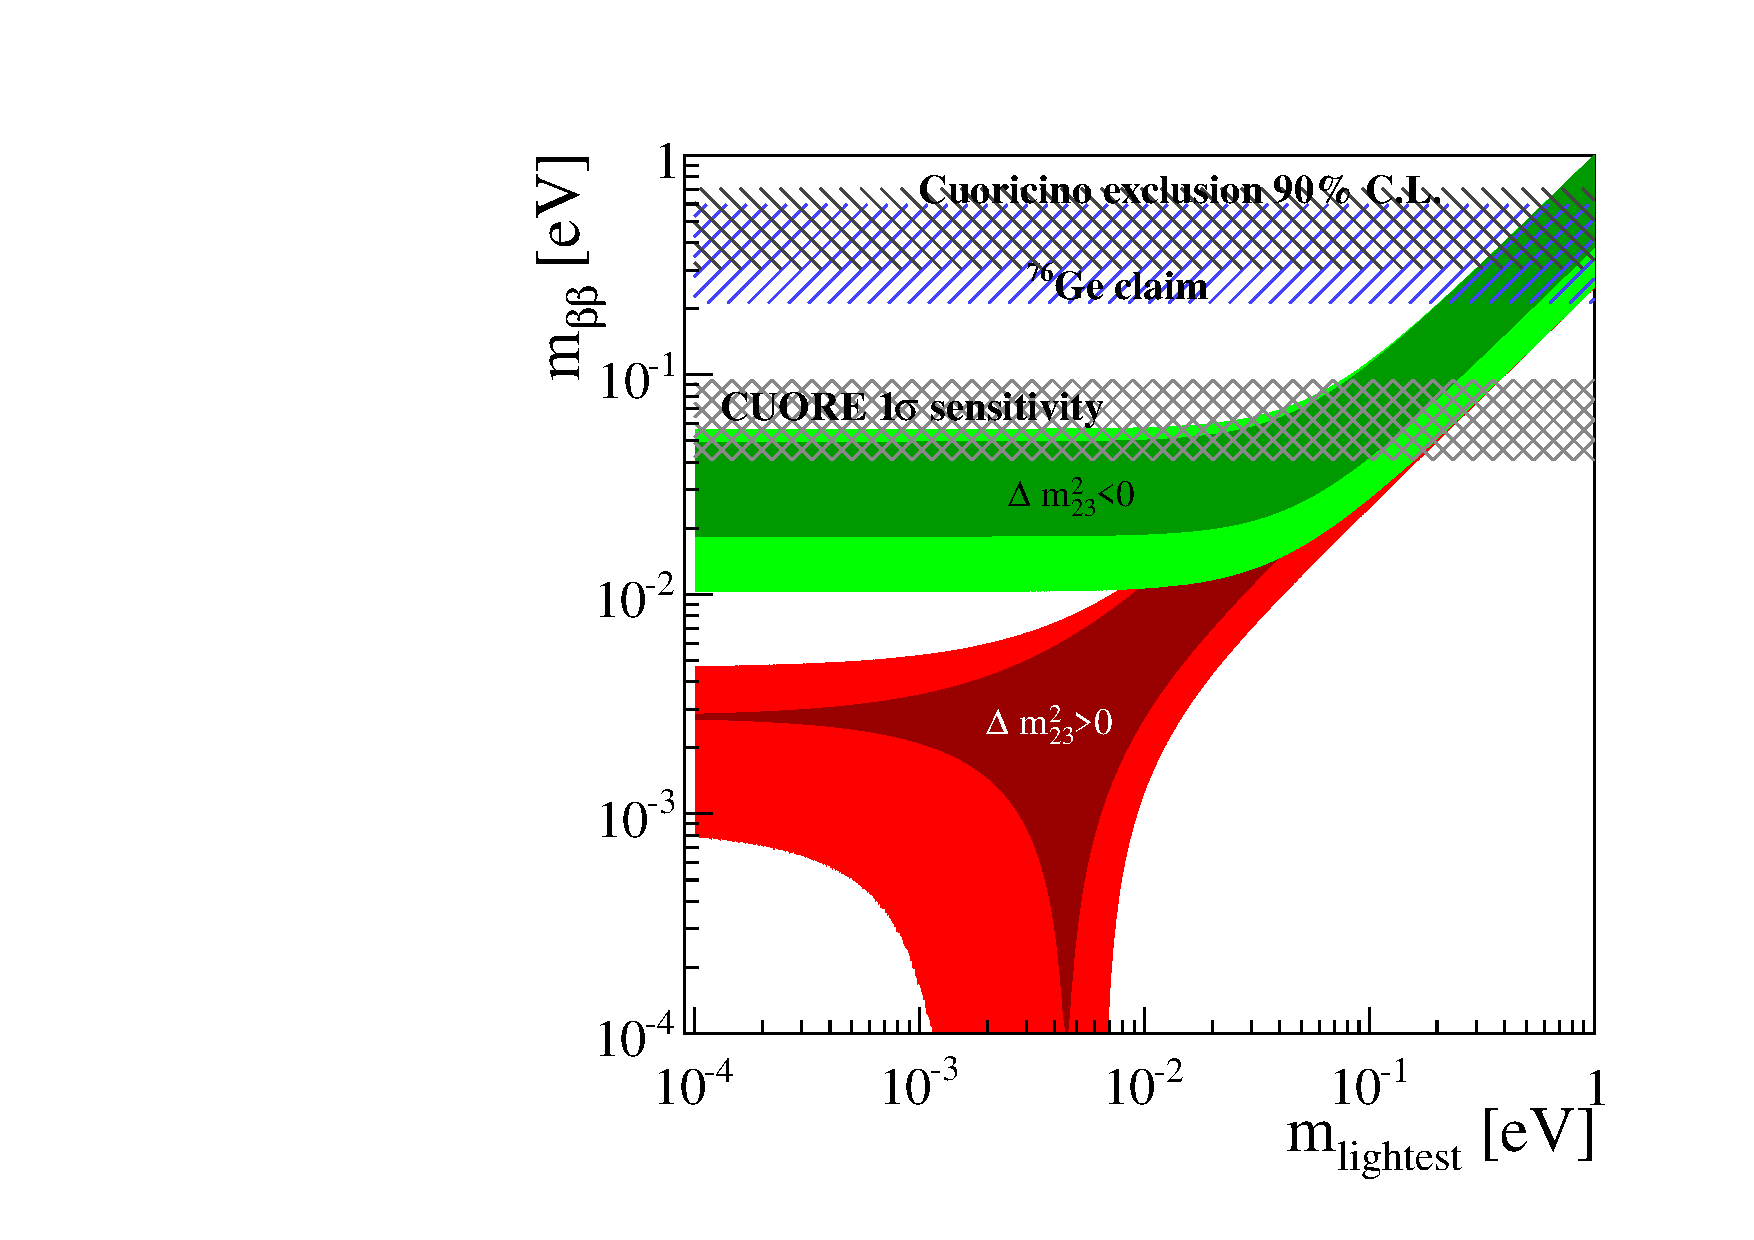
\includegraphics[width=0.45\columnwidth]{CUORE_Sensitivity.pdf} 
\end{center}
\caption{\label{sensCUORE}The sensitivity of the CUORE experiment as a function of the effective Majorana mass of the neutrino and the lightest neutrino mass eigenstate\cite{Alessandria:2011rc}. }
\end{figure}

As CUORE-0 runs, the rest of the towers will be constructed, and they will be installed by the end of 2014. The crystals are read out using Neutron Transmutation Doped (NTD) Ge thermistors. The assembly is labor-intensive, and one reason is that the NTDs are glued to each crystal individually. Therefore, All collaborators will be needed to help in this effort and for shift taking on CUORE-0. In parallel, the cryostat will be commissioned and integrated with the calibration system. The first test of this integration will take place this winter with the so-called ``4K'' test. The final configuration of the front-end electronics is being finalized now and everything is on schedule for data taking and first results from the full CUORE in 2015.

\subsection{Hardware Focus: Slow Monitoring}
The main components of the CUORE detector are the crystals, their electronics, the cryostat to cool the crystals to their 10~mK operating temperature, and the calibration system, which is a wire based system to move sources in and around the crystals. This is all being assembled in a three-story-hut,  Fig.~\ref{layoutCuore} (right), underground at the Laboratori Nazionali del Gran Sasso. Although Gran Sasso is one of the most convenient underground laboratories in which to work, access is not always guaranteed. For this reason, a robust remote monitoring system for all detector components and the surrounding environment is needed. The collaboration has identified this as a critical task within the project, which, as yet,  has not been assigned.

The task has two parts: unifying the slow monitoring and the interface to the data from the various devices that make up the detector, and providing hardware to monitor the environment in the three-story CUORE hut. For measuring the environment, a hardware package needs to be constructed which can measure temperature, humidity, and radon levels.  One package is needed on each of the three floors of the hut, in addition to one spare. A netbook per floor is envisioned for reading out the systems plus a rack-mounted computer devoted to slow monitoring to run the main database and serve the data. This is very similar to the package and system put together for Double Chooz. 

The proposed package uses inexpensive radon counters purchased from Aware Electronics\cite{aware} where the output pulses are then counted with the USB-CTR-15\cite{usbctr}.  The latter device has many spare channels for other devices from other systems that may need to be integrated into the slow monitor system. Unfortunately, the temperature and humidity sensors used on Double Chooz and KamLAND have been discontinued. There are several companies making TCP/IP-readable packages, ranging from \$60 to \$200 depending on the sophistication of the readout. Depending on the air-conditioning system, more thermometers may be needed, so the upper estimate is used in the budget summarized in Table~\ref{slowRequest}. In addition to the temperature and humidity sensors, other sensors such as accelerometers should be included in the design.

\begin{table}[position specifier]
\begin{center}
\begin{tabular}{ l c l}
\hline
Equipment & Number & Cost \\
\hline
Netbook & 4 & \$1500.00\\
USB-CTR-15 & 4 & \$1000.00\\
Temp. \& Humidity & 4 & \$800.00 \\
Other Sensors & 4 & \$800.00 \\
Radon Counter & 4 & \$1600.00\\
Slow Monitoring Server & 1 & \$4500.00 \\
\hline
Total & & \$11000.00 \\
\hline
\end{tabular}
\caption{\label{slowRequest}The budget for environmental monitoring for CUORE. The estimate for the slow monitoring server is from a recent purchase of a dual six-core 2.66Ghz 48GB system. Spares are requested to facilitate debugging at UCLA and allow for quick shipment to site. These costs are unloaded.}
\end{center}
\end{table}

The second half of this task is the centralization of the slow monitoring data. The most critical device to monitor is the cryostat, which is read out via LabVIEW. The calibration system and several other miscellaneous devices have internal TCP/IP servers for communication, while several older devices still communicate via RS232. The software package that manages these devices must have the infrastructure to build interfaces to these devices, provide infrastructure to process data and set alarms, and finally provide a user interface such as a graphical user interface (GUI) or a webpage for shift taking. This sort of software package is called a Supervisory Control And Data Acquisition package (SCADA). The PI has taken part in writing a custom SCADA package for Double Chooz. There are also several open-source packages that have been developed for operating physics experiments. Based on the PI's experience, an open source package is the more time-effective option.

The software packages that are being considered are EPICS\cite{epics}, MIDAS\cite{midas}, TANGO\cite{tango}, TINE\cite{tine}, and ORCA\cite{orca}.  Most of these packages come from the accelerator community, except for ORCA, which has been developed primarily for the Majorana program. ORCA is a Mac-based system, and at this point it may not be possible to port it to CUORE. On the other hand, EPICS is being used on MicroBooNE in addition to being used extensively on the LAr development at Fermilab; therefore, it has a large user community that overlaps with CUORE.

Evaluations of these software packages on a Debian-based Linux system were started this summer by two Italian collaborators, Andrea Giachero and Nicolo'o Moggi. They welcome additional man-power as both spend only a fraction of their time on CUORE. At UCLA, an undergraduate researcher, Walid Rahman, has joined the PI's group and will start running tests of the software packages locally.  The results of these evaluations will be discussed at the next collaboration meeting in October 2012, with the aim of having a prototype system available as early as this winter for the 4K integration test of the cryostat and calibration system.

\subsection{Analysis Focus: Monte Carlo and Exotic Double Beta-Decay Searches}
The great enthusiasm for double-beta decay searches comes from the fact that the observation of \zeronu~would prove that the neutrino is a Majorana particle. This has consequences for cosmology and models of leptogenesis, which use the heavy neutrino partners of light neutrinos to produce the matter-antimatter asymmetry in the universe. 
%There are also implications in the Higgs sector\cite{SVHiggs}, and the observation of \zeronu~could shed light on the properties of the Higgs boson that was recently discovered at ATLAS and CMS. 

The main CUORE analysis is the search for \zeronu~moderated by a light Majorana neutrino.  However, other models exist for the double-beta decay of Majorana neutrinos. One group involves the ejection of a massless boson called a Majoran $\chi^{0}$. The observational signature of these models (\maj) is a change in the detected summed energy of the two electrons, as shown in Fig.~\ref{majoran}.  In the models where the decay is moderated by a light Majorana neutrino, the sum of the electron energy is the endpoint energy broadened by the detector resolution. The \maj~models show a broadened spectrum corresponding to the sharing of the energy among the electrons and the $\chi^{0}$. 

\begin{figure}
\begin{center}
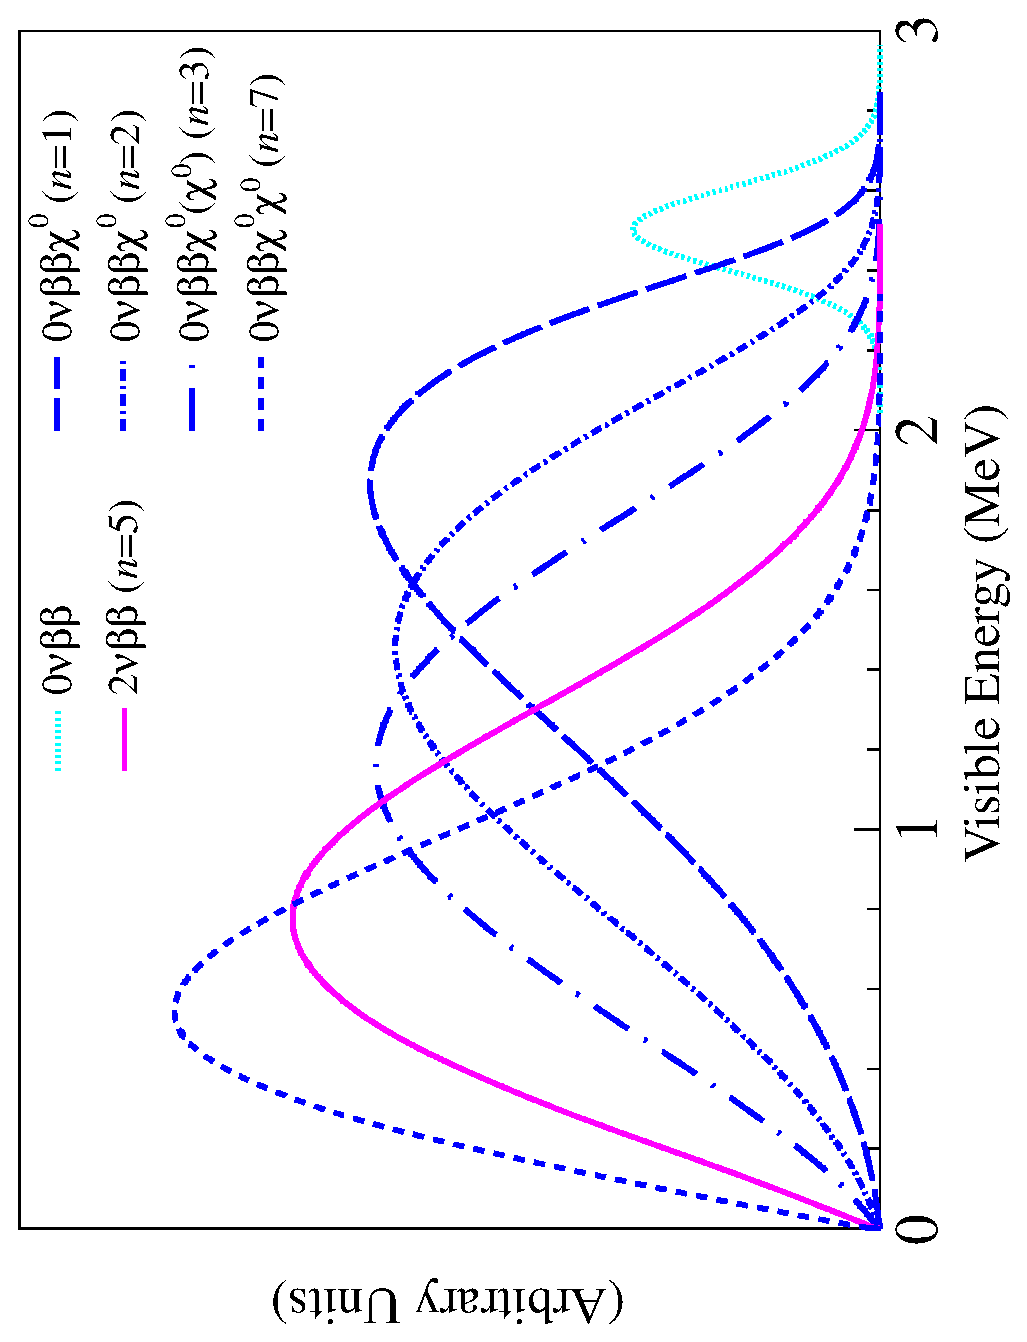
\includegraphics[angle=270, width=0.58\columnwidth]{fig1} 
\end{center}
\caption{\label{majoran}The effect of Majoran emission on the \zeronu~spectrum from Ref.~\cite{KZMaj}. The endpoint for \isoxe~is shown. The search in CUORE would be the same except centered at the \isomain~endpoint of 2.527~MeV. }
\end{figure}

The best limits on these models currently come from the KamLAND-Zen experiment, which puts limits on the half-lives in \isoxe~of $T_{1/2}^{0\nu\chi^0}>2.6\times10^{24}$~yrs at the 90\% C.L.\cite{KZMaj}. The best limits on this process in \isomain~are $T_{1/2}^{0\nu\chi^0}>1.6\times10^{22}$~yrs at the 90\% C.L. from the NEMO-3 experiment\cite{nemo3Te}. NEMO-3 is a tracking detector which allows for large reductions in backgrounds. Unfortunately, the measurement was still limited by backgrounds and had a signal to noise (S/N) of 0.5. CUORICINO did not search for these processes.

The measurement of the standard model process of two-neutrino double-beta (\twonu) is closely related to the $\chi^{0}$ search and is a background to the search. The \twonu~analysis was the thesis topic of the CUORICINO student Laura Kogler\cite{laura}. The background levels in CUORICINO were too high to extract the \twonu~rate by directly simulating and fitting the background shapes. In order to extract \twonu~half-life, a background subtraction was done using crystals depleted in~\isomain. This type of subtraction will not be possible in CUORE since there are no plans to run with crystals of different enrichments. The reduced background contamination is expected to bring the S/N up to 1.0. At this background level, a fit should be possible by directly simulating the background shapes. This would allow an improved measurement of the \twonu~rate, and a search for double-beta decay with $\chi^{0}$ ejection. In addition, the \twonu~measurement is interesting in itself as it can be used to understand the quality of the different nuclear matrix calculations. 

The search for \maj~complements the main \zeronu~analysis because it requires a detailed model of the backgrounds and detector response in a larger section of the detected spectrum. This analysis builds on the PI's analysis strengths in simulating and fitting background spectra in low-energy neutrino experiments. In fact, the analysis of the data is almost identical to the \zeronu~search the PI is leading on Double Chooz. It also carves out searches for exotic double-beta decay modes as the physics focus for the group and this proposal.

%This is the low background paper, not going to use it?
%\cite{Alessandria:2012ha}

\subsection{Group Plan}
This proposal's purpose is to support the participation of the PI, a postdoc, one undergraduate, and one graduate student on CUORE. The general plan for the group is the slow monitoring work in the first year of the award, commissioning in the second year, and data analysis in the third year of the award. The undergraduate researcher, Walid Rahman, has already started working on the slow monitoring. He is a junior transfer student and will be at UCLA for year one and year two of the award. In year two of the grant, a younger student will be recruited for year three. 

The entering class of graduate students at UCLA in 2012 was small, and therefore it is unlikely that the PI will find a graduate student before the start of the grant. Instead the PI would prefer to recruit a graduate student from the incoming group in 2013. The PI is particularly interested in recruiting one of three undergraduate researchers with CUORE experience who will graduate from Cal Poly San Luis Obispo this year. In year one and two of the grant, this student would be taking class; therefore, they would spend the summers onsite working on tower construction, taking CUORE-0 shift, and generally becoming an expert on the detector and CUORE-0 data analysis. During the academic year at UCLA, they would write the \maj~MC generator, and learn how to run the CUORE MC at UCLA's computing facility. In year three of the award, they should be ready to assist the postdoc with the search for \maj~ in the full CUORE data.

The postdoc is the critical member of the group. The integration of the slow monitoring needs a person to spend at least 50\% of their time onsite during the first year of the award to facilitate this process and to understand the needs of the detector as it is constructed. As one of the goals is to build an analysis group at UCLA, the postdoc will not be stationed onsite. Because of the low-level nature of the hardware work, a postdoc with experience in \zeronu~physics is preferred, so that they may  jump into the analysis quickly.  In addition to a general search, two candidates who could start in January have been identified, and are being recruited. This advertisement should be posted shortly. 

In the first year of the award, the postdoc will need to focus on the slow monitoring, but some time should be used to develop code to do the basic sensitivity study for the \maj~search. The second year of the award represents the apex of the CUORE commissioning, and the postdoc should be in the heart of this effort as the leader of the slow monitoring and a member of the UCLA electronics group. In this time, the results of the basic sensitivity study should be used to guide the background simulation efforts. The third year of the grant should have the first data from the full CUORE detector, and the analysis ready to run. The postdoc should be ready with the simulated backgrounds and should be in a good position to be a leader in the main analysis as well as the search for \maj. Most critically, this should also provide the postdoc the results that are needed for applying for a job in that year or the following one.

In addition to the support for CUORE, the PI requests travel funds to complete their Double Chooz work in the first year of the award, and travel funds to nurture future experiments at KamLAND through the whole award. This would consist of two international and one domestic trip per year of the grant. Studies for these future experiments are nice projects for undergraduates; therefore, support is requested for a second undergraduate, Ruben Gutierrez Martinez, to study backgrounds for a proposed sterile neutrino search at KamLAND\cite{isodar}. Gutierrez is a joint physics and computer science major so this simulation project is a good match to his interests.

\section{Broader Impacts}
\subsection{CUORE:  The Search for Neutrinoless Double-Beta Decay}
\begin{figure}
\begin{center}
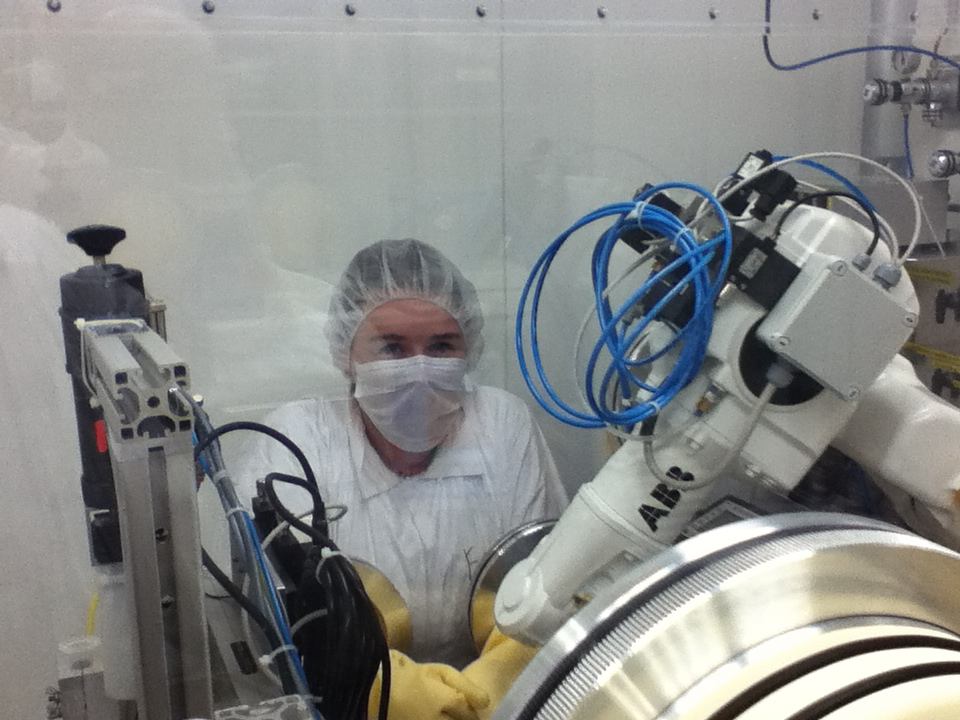
\includegraphics[width=0.35\columnwidth]{figs/Erin1.jpg} 
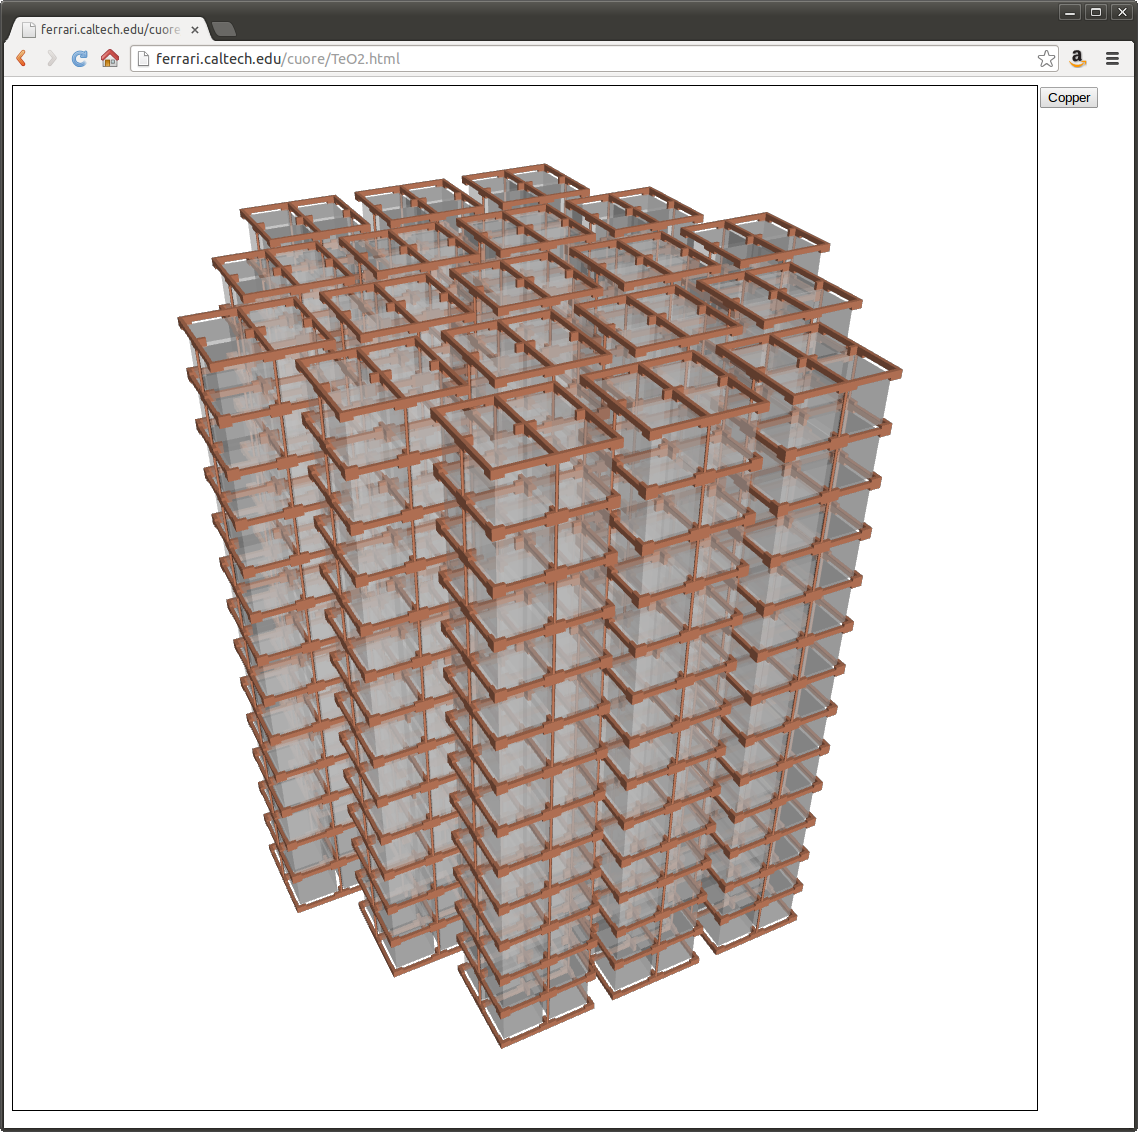
\includegraphics[width=0.3\columnwidth]{figs/viewerPlain.png} 
\end{center}
\caption{\label{broad} (Left) Graduate student Erin Hansen gluing thermistors as the gluing leader during the summer of 2013. (Right) Web-based visualization of the CUORE Monte Carlo. A series of button will allow the highlighting of different detector components and in the future will allow the creation of an event viewer for public outreach. }
\end{figure}

The broader impacts of this proposal are three-fold: training of students in nuclear physics, broadening the diversity of participation in physics, and public outreach through a web-based event viewer. The CUORE experiment provides training in nuclear physics for graduate and undergraduate students. The Nuclear Science Advisory Committee (NSAC) report on education in nuclear science from 2004 recommended a 20\% increase in the number of students trained in nuclear physics over the next 10 years to meet the needs of the U.S. workforce\cite{nuced}. The connection between the double-beta decay measurement and astronomy and cosmology captures the imagination of students and draws them into nuclear science, where they can learn why this is such an exciting field of study.The graduate student who will be supported by this grant is shown in Figure~\ref{broad}.

Secondly, the PI has a long track record of working to increase the participation of women
and minorities in physics. The PI's mentoring work with the MIT Summer Research Program was recognized with MIT"s Infinite Kilometer Award. The PI continues this work with enthusiasm at UCLA. The requested funds for two undergraduate students will give more undergraduates the opportunity to experience both the direct and indirect benefits of research. These students will takeover from current undergraduates Elizabeth Friedman on CUORE and Ruben Gutierrez on the IsoDAR proposal. The PI has advises fledgling graduate and undergraduate women in physics groups. Friedman is the founder of the undergraduate women's group and we are working together to arrange monthly lunches and for a group of UCLA undergraduates to attend the undergraduate women in physics hosted at UC Berkeley this winter.

%and mentored Athena Ierokomos as part of UCLA's REU program.
The third impact of this proposal will be the creation of a website explaining the CUORE experiment and its results for the public. The center piece of this website will be an interactive event viewer based upon the visualization of the CUORE Monte Carlo. A screenshot of the web-based viewer with one button to highlight the copper support is shown in Figure~\ref{broad}. The PI has worked on similar projects most recently a online course on neutrino oscillations as part of the Annenberg Foundation's \textit{Physics for the 21$^{st}$ Century}. 

The success of the broader impacts of this grant will be demonstrated in several ways.   First, by the end of the three-year grant, the goal is to ensure the new women in physics groups at UCLA have active ongoing programs.  Second, success will be defined by maintaining a diverse group and continuing to recruit minority students to the group. Currently, UCLA has a 10\% minority population within the physics major in which to advertise. However, one of UCLA's great strengths is its large hispanic community, 17\% of the undergraduate population. This represents a great recruiting opportunity for increased participation in the major. The success  of these students will be defined by the publication of papers and presentations at  conferences like APS April Meeting. We are excited to note that  Gutierrez obtained one of the Conference Experience for Undergraduate slots at DNP2013 and will be presenting his IsoDAR work there. Finally by the end of the award, a website for the public will be complete, centered around the interactive event display.

\section{Conclusion}
The neutrino is not quite as mysterious as it was a decade ago, but the physics questions are arguably more important. The first detection of neutrinoless double-beta decay will have great implications for mass generation in particle physics, but the ripples from such a discovery will be felt in the far corners of astrophysics and cosmology. The CUORE  detector is poised to probe deeper into the double-beta decay parameter space than any experiment that will turn on in the next few years, and its technology of TeO$_2$ bolometers is applicable to other measurements.

This technology is new to the PI, but their experience in other low background physics has prepared them well for this analysis. Specifically in the last two years, the PI has been one of the coordinators of the Double Chooz  analysis which has produced five analysis papers related to reactor antineutrinos and the measurement of $\theta_{13}$\cite{dcone, dctwo, takahama,Abe:2012gw,Abe:2012ar}. This work continues with several papers in progress including a search for \zeronu~in $^{160}$Gd. In this same period, the PI has also published several papers related to R\&D efforts and proposals for new experiments\cite{Alonso:2010fs,isodar,qdot,Lopez201222}.

This award mainly supports students and a postdoc on CUORE. The group's proposed hardware task of the slow monitoring builds on the PI's slow monitoring experience on Double Chooz and integrates the group with the greater CUORE effort. Similarly, the proposed analysis focus on searches for exotic double-beta decay modes builds on the PI's experience simulating backgrounds, gives the group a well defined task, but does not segregate the group from the main CUORE analysis. 

It is an exciting period for CUORE as the pieces are coming together, and data from the completed detector is on the horizon. This is a great time for a new group to join the experiment, especially one that has support at their home institution and in the greater collaboration. The PI is knowledgable in the field and is well positioned to lead a group towards interesting new physics. 
